\documentclass[12pt]{article}
\usepackage{subcaption}
\usepackage[spanish]{babel}
\usepackage{pgfplots}
\usepackage[utf8]{inputenc}
\usepackage{amsmath,amssymb,amsthm}
\usepackage{graphicx,float}
\usepackage{cancel}
\graphicspath{ {fotos/} }
\providecommand{\abs}[1]{\lvert#1\rvert}
\providecommand{\norm}[1]{\lVert#1\rVert}
\usepackage[a4paper, left=3cm, right=3cm, top=35mm, bottom=20mm]{geometry}
\usepackage{blindtext}
\usepackage{graphicx}
\usepackage[backend=biber,style=apa,natbib=true]{biblatex}
\addbibresource{referencias.bib}
\setlength\bibitemsep{1.5\itemsep}
\usepackage{adjustbox}
\usepackage[hidelinks]{hyperref}

\begin{document}

\begin{titlepage}
\begin{center}
{\scshape\huge Física e instrumentación espacial \par}
\vspace{1cm}
{\scshape\Large Cálculo numérico \par}
\vspace{1cm}
{\textbf{{\Huge Resolución Numérica de la Ecuación de Schrödinger}} \par}
\vspace{1.5cm}
{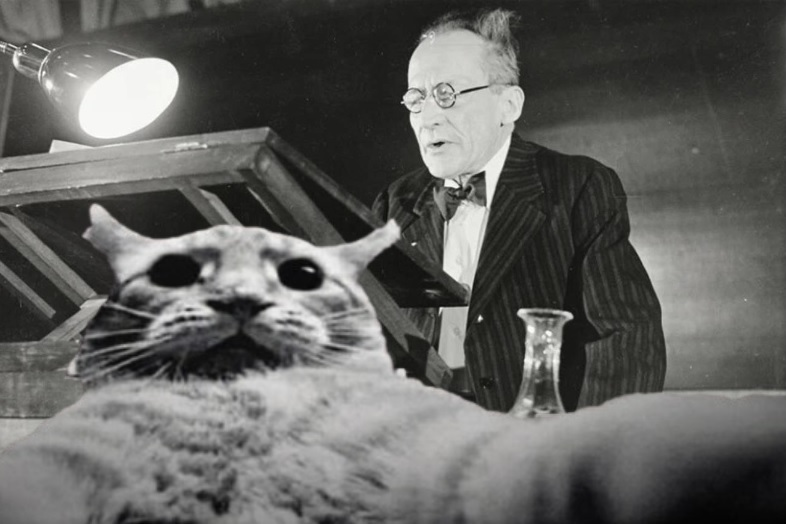
\includegraphics[scale=0.8]{portada.jpg}\par}
\vspace{1cm}
{\scshape\Large Abril 2024 \par}
\vspace{1.5cm}
\end{center}
\begin{flushleft}
{\Large Autores: \par}
{\Large 
Víctor Ávila Camargo\\
José Ignacio Miguel Rodríguez\\
Javier Zaragozano Calvo \par
}
\end{flushleft}
\end{titlepage}

\tableofcontents
\newpage	

\section{Introducción}
La ecuación de Schrödinger es una de las ecuaciones más famosas
e importantes de la Física Cuántica. La ecuación de Schrödinger en una dimensión en su forma más general es: 
\begin{equation}
i\hbar \frac{\partial}{\partial t}\Psi (x,t)=\hat{H} \Psi (x,t)
\end{equation}
Donde $\hat{H}$ es el Hamiltoniano del sistema. \\
\par
Esta ecuación tiene numerosas variantes. En este artículo, nos 
centraremos en resolver una de sus variantes, la ecuación de Schrödinger
independiente del tiempo que, como su propio nombre indica, el tiempo
no aparece como variable independiente. Esta ecuación se puede obtener a partir de la ecuación descrita arriba, veámoslo.


\subsection{Deducción de la ecuación de Schrödinger independiente del tiempo}
Sea el Hamiltoniano de un sistema cualquiera: 
$\hat{H}=-\frac{\hbar^{2}}{2m}\frac{\partial^{2}}{\partial x^{2}}+V(x,t)$.
Si consideramos que es independiente del tiempo, $V(x,t)$ tiene que ser también 
independiente del tiempo ya que es el único término del Hamiltoniano
con dependencia temporal. Con lo cual $\hat{H}=-\frac{\hbar^{2}}{2m}\frac{\partial^{2}}{\partial x^{2}}+V(x)$ \\
\par
Nuestro objetivo es dejar un lado de la ecuación en función de t y el otro en función de x. Al ser una ecuación diferencial, vamos a usar el método de separación de variables. Entonces, considerando las soluciones estacionarias para la ecuación obtenemos: $\Psi (x,t)= g(t) \psi(x)$. Por tanto, nos queda:

\begin{equation*}
i\hbar \psi (x) \frac{d}{d t}g(t)= g(t) \hat{H} \psi (x)
\end{equation*}

Como el Hamiltoniano es independiente del tiempo podemos mover libremente  $g(t)$ porque no va a operar sobre él. Multiplicando ambos  lados por $\frac{1}{g(t)\psi(x)}$ obtenemos:

\begin{equation*}
i\hbar \frac{1}{g(t)} \frac{d}{d t}g(t) = \frac{1}{\psi(x)} \hat{H} \psi (x)
\end{equation*}

Como cada lado depende de una variable distinta, la igualdad
se cumplirá sí y solo sí el resultado es igual a una constante la cual llamaremos E. Entonces por un lado tenemos:

\begin{equation*}
\frac{d}{d t}g(t)=-\frac{i}{\hbar} Eg(t)
\end{equation*}

Obteniendo como solución:

\begin{center}
    $g(t)= e^{-\frac{i}{\hbar}Et}$
\end{center} 

Considerando estos resultados, llegamos a la siguiente forma para nuestra ecuación:

\begin{equation}\label{eq:ESROW}
\left(-\frac{\hbar^{2}}{2m}\frac{d^{2}}{d x^{2}}+V(x)\right) \psi(x)=E \psi(x)
\end{equation}

Esta es la \textbf{Ecuación de Schrödinger independiente del tiempo} y es la que nos centraremos en resolver en este artículo. 
La ecuación se puede abreviar del siguiente modo: $\hat{H} \psi (x)=E \psi (x)$ y vemos
que es un problema de autovalores donde $E$ se corresponde con el autovalor de $\hat{H}$. \\

Sin embargo, resolver esta ecuación no es trivial y, 
por ello, será necesario emplear métodos numéricos, 
los cuales serán descritos en detalle en las secciones posteriores, para encontrar una solución aproximada. \\

Una inquietud que le puede surgir al lector es qué interpretación
tiene las soluciones que se obtengan. Así que vamos a intentar esclarecer esta duda en el siguiente apartado.

\subsection{Interpretación de la ecuación de Schrödinger y sus soluciones}

Las soluciones que obtenemos son funciones de onda que van asociadas a la partícula que queremos describir. Esto es debido a la dualidad onda-partícula que caracteriza a todas las partículas del Universo. Sin embargo, no podemos ver estas funciones de onda del modo clásico, tenemos que verlas como
funciones de probabilidad que nos indican en qué zonas es más probable que se encuentre nuestra partícula. Esta función de probabilidad se puede describir como: 

\begin{center}
    $dP(x,t)=\left\lvert \Psi (x,t) \right\rvert^{2} dx$
\end{center}

Esto es la probabilidad de encontrar la partícula en un fragmento de espacio infinitesimal. Al ser una función de probabilidad cumple que:

\begin{equation}\label{eq:norm}
    \int_{espacio} \left\lvert \Psi (x,t) \right\rvert^{2} \,dx=1
\end{equation}

Por otro lado, también encontramos valores de E asociados a la función y al Hamiltoniano. Para ver lo que significan las E que obtenemos, vamos a calcular el valor esperado de $\hat{H}$:

\begin{align*}
\langle \hat{H} \rangle_{\Psi (x,t)} \notag 
&=\int \Psi (x,t)^{*} \hat{H} \Psi (x,t) \,dx= \notag \\
&=\int \Psi (x,t)^{*} E \Psi (x,t) \,dx= E
\end{align*}

Por definición del valor esperado de $\hat{H}$, sabemos que representa la  energía total del sistema. Es decir, los autovalores que obtengamos al resolver la ecuación nos darán un valor para la energía del sistema. \\

Una vez hechas todas estas aclaraciones introductorias, ya podemos
comenzar con la descripción de todos los métodos numéricos y 
también podemos ver las soluciones obtenidas.

\newpage
\section{Métodos de derivación numérica}

\subsection{Método de las diferencias finitas}

El método de las diferencias finitas (FDM) es un método de aproximación para resolver ecuaciones diferenciales. Su principio fundamental es transformar una ecuación diferencial en un sistema de ecuaciones algebraicas que podamos resolver. El principio del método de diferencias finitas fue desarrollado por primera vez por el excelentísimo matemático L. Euler (1707-1783), quien en 1768 dio un formato diferencial para problemas unidimensionales. En 1908, C. Runger (1856-1927) extendió el método de la diferencia a problemas bidimensionales. Sin embargo, en aquellos días, convertir la solución de ecuaciones diferenciales en la solución de un gran número de ecuaciones algebraicas era sin duda transformar un problema en otro, por lo que no se usaba ampliamente. Con el desarrollo de la tecnología informática, es posible resolver de forma rápida y precisa enormes ecuaciones algebraicas, por lo que poco a poco se ha ido generalizando su uso.\\

Este método nos será de gran utilidad si queremos resolver la ecuación de Schrödinger:

\begin{equation*}
\frac{\hbar^2}{2m} \frac{\partial^2\psi}{\partial x^2} + V(x)\psi = E \psi
\end{equation*}

Nada más y nada menos que en el primer término ya nos encontramos una derivada segunda, lo que convierte nuestro problema en resolver una ecuación diferencial. Nuestro objetivo entonces será aproximar esta derivada por el método propuesto para poder obtener soluciones de la misma. Más tarde, estudiaremos el impacto de realizar esta aproximación y el error que conlleva aplicarla.\\

El método de diferencias finitas consiste en discretizar el espacio en el que estemos trabajando y así transformar la distancia infinitesimal entre puntos de las derivadas en una distancia $h$. Por tanto, dividimos $N$ veces, un intervalo $[a,b]$, donde la función es continua. El espacio entre los puntos que nos queden lo llamaremos distancia de paso ($h$) y el tamaño de este nos dará la precisión de nuestra aproximación como veremos más adelante.\\

\newpage
Este concepto puede hacerse más sencillo de comprender al ver la siguiente figura:

\begin{figure}[H]
\centering
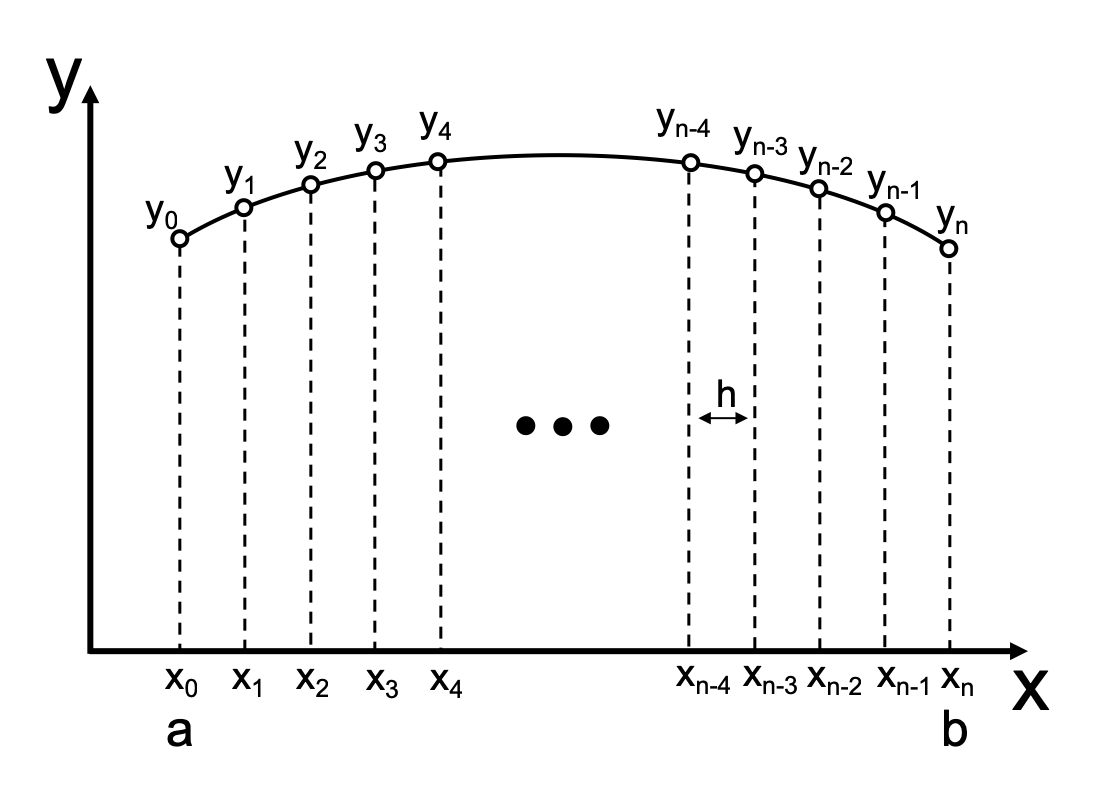
\includegraphics[width=4in]{23.03.01-Finite-difference}
\caption{Discretización del espacio con paso h.}
\label{finite_difference}
\end{figure}


\subsubsection{Diferencial de primer orden}

Para obtener una aproximación de la diferenciación en este nuevo espacio lo que nos viene a la mente es la definición de derivada, que la aproximaremos de la siguiente manera:

\begin{equation}\label{eq:eq1}
u'(x)=\lim_{h \to 0}  \frac{u(x+h)-u(x)}{h} \approx \frac{u(x+h)-u(x)}{h}
\end{equation}

\begin{figure}[H]
    \centering
    \begin{adjustbox}{width=1.15\linewidth,center}
        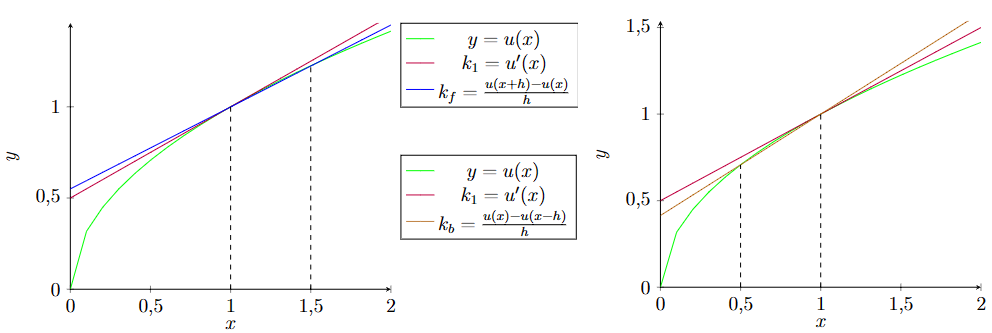
\includegraphics{fotos/dffttudo.png}
    \end{adjustbox}
    \caption{En el lado izquierdo, derivada forward de la función $\sqrt{x}$ en el punto x=1. A la derecha, misma situación pero usando derivación backward.}
    \label{fg:ttudo}
\end{figure}

La recta roja corresponde a la derivada de la función $\sqrt{x}$ en el punto $x=1$,
mientras que la recta azul corresponde a la de nuestra aproximación con paso $h=1$.
Como se puede observar es realmente parecido y según hagamos el paso más pequeño 
esta diferencia se hará menor.\\

Se nos puede ocurrir otra aproximación de la derivada, en vez de aproximarlo con el punto siguiente podríamos tratar de aproximarlo con el punto anterior (imagen del lado derecho de la figura~\ref{fg:ttudo}).\\

Por lo tanto, aquí primero necesitamos discretizar el dominio de la solución y luego obtener la aproximación diferencial en cada punto discreto por separado. Para el problema unidimensional dividimos el intervalo de la solución en partes iguales.\\

La forma discreta de la ecuación (\ref{eq:eq1}) se expresa como: 								
\begin{equation}
u'_i(x)=\frac{1}{h}(u_{i+1} - u_i)
\end{equation}
y la misma, pero utilizando el punto anterior y no el siguiente:
\begin{equation}
u'_i(x)=\frac{1}{h}(u_i-u_{i-1})
\end{equation}
Demostraremos ahora de donde salen estas fórmulas que tan hábilmente se nos han ocurrido.\\

Para la derivada de primer orden, si aproximamos por Taylor:

\begin{equation*}
u(x+h)=u(x) + hu'(x)+ \frac{h^2}{2}  u''(x)+ \frac{h^3}{6} u^{(3)}(x+\xi) 
\end{equation*}

donde $\xi\in (0,h)$. La fórmula de la derivada forward para el diferencial de primer orden se puede obtener deformando la ecuación anterior:

\begin{equation*}
u_F'(x)=\frac{u(x+h)-u(x)}{h} - \frac{h^2}{2}u''(x+\xi)
\end{equation*}

Ahora si aproximamos por Taylor $u(x-h)$:

\begin{equation}
u(x-h)=u(x) - hu'(x)+ \frac{h^2}{2}  u''(x) - \frac{h^3}{6} u^{(3)}(x+\xi)
\end{equation}

donde $\xi\in (0,h)$, si modificamos la ecuación de forma similar al caso anterior obtenemos:

\begin{equation}
u_B'(x)=\frac{u(x)-u(x-h)}{h} + \frac{h^2}{2}u''(x+\xi)
\end{equation}

Si juntamos ambas ecuaciones obtenemos la fórmula de la diferencia central para el diferencial de primer orden

\begin{equation}
u_C'(x)=\frac{u(x+h)-u(x-h)}{2h} - \frac{h^2}{6}u^{(3)}(x+\xi)
\end{equation}

Dado que el error aquí es relativo al tamaño del paso, se puede ver que las fórmulas de la diferencia hacia adelante y hacia atrás tienen una precisión de aproximación de primer orden $O(h)$, mientras que la diferencia central tiene una precisión de aproximación de segundo orden $O(h^2)$. Es por esto que nos interesa juntar ambas ecuaciones (cuanto mayor sea el orden, antes tiende el error a cero).\\

Para el caso anterior obtendríamos la siguiente aproximación:

\begin{figure}[H]
\centering
\begin{tikzpicture}[scale=1]
\begin{axis}[
axis lines = left,
xlabel = $x$,
ylabel = {$y$},
legend pos=outer north east,
xmin=0, xmax=2,
]
\addplot [
domain=0:10, 
samples=100, 
color=green,
]
{sqrt(x)};
\addlegendentry{$y = u(x)$}

\addplot [
domain=0:10, 
samples=100, 
color=purple,
]
{0.5*x + 0.5};
\addlegendentry{$k_1 = u'(x)$}

\addplot [
domain=0:10, 
samples=100, 
color=red,
]
{0.51763*x + 0.4142};
\addlegendentry{$k_c = \frac{u(x+h)-u(x-h)}{2h}$}

\draw[dashed] (axis cs:1,0) -- (axis cs:1,1);

\end{axis}
\end{tikzpicture}
\caption{Derivada central de la función $\sqrt{x}$ en el punto x=1.}
\end{figure}

Vemos como la pendiente de las rectas es mucho más similar que en los casos anteriores, por tanto, es coherente con nuestra demostración sobre la precisión de esta nueva aproximación de la derivada.

\subsubsection{Diferencial de segundo orden}

Para nuestra ecuación, sin embargo, no necesitamos obtener una aproximación de la derivada de primer orden si no de la de segundo orden. Por tanto, trabajaremos ahora con la demostración de esta.\\

Como anteriormente realizamos la expansión de Taylor:

\begin{equation*}
u(x+h)=u(x) + hu'(x)+ \frac{h^2}{2}  u''(x) + \frac{h^3}{6} u^{(3)}(x)+\frac{h^4}{12}u^{(4)}(x+\xi)
\end{equation*}

Pasando el término u''(x) a la derecha obtenemos:

\begin{equation}
u_F''(x)=-\frac{2u(x)}{h^2} - \frac{2u'(x)}{h} - \frac{h}{3}u^{(3)}(x)-\frac{h^2}{6}u^{(4)}(x+\xi) {h^2} + \frac{2u(x+h)}{h^2}
\end{equation}

De igual manera  obtenemos:

\begin{equation*}
u(x-h)=u(x) - hu'(x)+ \frac{h^2}{2}  u''(x) - \frac{h^3}{6} u^{(3)}(x)+\frac{h^4}{12}u^{(4)}(x+\xi)
\end{equation*}

\begin{equation}
u_B''(x)=-\frac{2u(x)}{h^2}  + \frac{2u'(x)}{h} + \frac{h}{3}u^{(3)}(x)-\frac{h^2}{6}u^{(4)}(x+\xi) {h^2} + \frac{2u(x-h)}{h^2}
\end{equation}
Juntando ambas obtenemos:
\begin{eqnarray*}
\frac{1}{2}(-\frac{2u(x)}{h^2} - \cancel{\frac{2u'(x)}{h}} - \cancel{\frac{h}{3}u^{(3)}(x)}-\frac{h^2}{6}u^{(4)}(x+\xi) {h^2} + \frac{2u(x+h)}{h^2} -\frac{2u(x)}{h^2} + \\ + \cancel{\frac{2u'(x)}{h}} +\cancel{\frac{h}{3}u^{(3)}(x)}-\frac{h^2}{6}u^{(4)}(x+\xi) {h^2} + \frac{2u(x-h)}{h^2}) \rightarrow
\end{eqnarray*}
\begin{equation}
\rightarrow u_C''(x)=\frac{u(x+h)-2u(x)+u(x-h)}{2h^2} - \frac{h^2}{6}u^{(4)}(x+\xi)
\end{equation}

Donde volvemos a apreciar que tenemos una precisión de aproximación de segundo orden relativa al tamaño del paso $(O(h^2))$.

\subsubsection{Error de aproximación en el método de las diferencias finitas}

Si recopilamos los errores de este método de derivación numérica obtenemos:

\begin{flushleft}
-Derivada de primer orden: diferencia ordinaria: 
$E \leq \frac{M_2}{2}h \sim O(h)$\\ donde $M_2 = \smash{\displaystyle\max_{x \in [x_0,x_0+h]}} |f''(x)|$
\end{flushleft}

\begin{flushleft}
-Derivada de primer orden: diferencia central: 
$E \leq \frac{M_3}{6}h^2 \sim O(h^2)$\\ donde $M_3 = \smash{\displaystyle\max_{x \in [x_0-h,x_0+h]}} |f'''(x)|$
\end{flushleft}

\begin{flushleft}
-Derivada de segundo orden: diferencia ordinaria:
$E \leq \frac{M_4}{12}h^2 \sim O(h^2)$\\ donde $M_4 = \smash{\displaystyle\max_{x \in [x_0-h,x_0+h]}} |f^{(4)}(x)|$
\end{flushleft}




\subsection{Aproximación de la ecuación de Schrödinger}
Si ahora aplicamos esto a la Ecuación de Schrödinger que ya habíamos escrito previamente: ecuación~\eqref{eq:ESROW}, podemos sustituir la derivada segunda por nuestra aproximación, quedando de la siguiente manera:

\begin{equation}
-\frac{\hbar^2}{2m} \frac{\psi_{i+1}(x)-2\psi_i(x)+\psi_{i-1}(x)}{h^2} + V_i(x)\psi_i = E \psi_i(x)
\end{equation}

Ahora debemos determinar un intervalo $[a,b]$ que será la región donde resolveremos 
la ecuación. Esta región la dividiremos en N+1 puntos, resultando en N subintervalos y siendo $h$ la longitud de estos.\\

El valor de la función en $x_0$ y en $x_n$ será 0, ya que la partícula estará confinada en dicho intervalo. Esto será lo que nos dará nuestras condiciones de frontera. Así pues, tendremos que resolver la función en los N-1 puntos restantes.

Nuestra matriz de energía cinética será:

\begin{equation*}
T=\frac{-\hbar^2}{2m} \left(
\begin{matrix}
\frac{-2}{h^2} & \frac{1}{h^2} & 0 & 0 &  \cdots & 0 \\
\frac{1}{h^2} & \frac{-2}{h^2} & \frac{1}{h^2} & 0 & \cdots & 0\\
0 & \frac{1}{h^2} & \frac{-2}{h^2} & \frac{1}{h^2} & \cdots & 0\\
\vdots & \vdots&\ddots &\ddots &\ddots& \vdots \\
0 & 0   &\cdots &\frac{1}{h^2}& \frac{-2}{h^2} & \frac{1}{h^2} \\
0 & 0 & 0  &\cdots & \frac{1}{h^2} & \frac{-2}{h^2} \\
\end{matrix}
\right)
\end{equation*}

Mientras que la de energía potencial será:

\begin{equation*}
V= \left(
\begin{matrix}
V_1 & 0 & 0 & 0 &  \cdots & 0 \\
0 & V_2 & 0 & 0 & \cdots & 0\\
0 & 0 & V_3 & 0 & \cdots & 0\\
\vdots & \vdots&\ddots &\ddots &\ddots& \vdots \\
0 & 0   &\cdots &0& V_{n-1} & 0 \\
0 & 0 & 0  &\cdots & 0 & V_{n} \\
\end{matrix}
\right)
\end{equation*}

Construimos nuestra matriz Hamiltoniana de la siguiente forma:
\begin{equation*}
H=T+V
\end{equation*}
Haciendo esto obtenemos el siguiente sistema lineal: \\

\begin{equation*}
\frac{-\hbar^2}{2m} \left(
\begin{matrix}
\frac{-2}{h^2} & \frac{1}{h^2} & 0 & 0 &  \cdots & 0 \\
\frac{1}{h^2} &  \frac{-2}{h^2} & \frac{1}{h^2} & 0 & \cdots & 0\\
0 & \frac{1}{h^2} &  \frac{-2}{h^2} & \frac{1}{h^2} & \cdots & 0\\
\vdots & \vdots&\ddots &\ddots &\ddots& \vdots \\
0 & 0   &\cdots &\frac{1}{h^2}&  \frac{-2}{h^2} & \frac{1}{h^2} \\
0 & 0 & 0  &\cdots & \frac{1}{h^2} &  \frac{-2}{h^2} \\
\end{matrix}
\right)
\left(
\begin{matrix}
\psi_1 \\
\psi_2 \\
\psi_3 \\
\vdots\\
\psi_{n-1} \\
\psi_{n} \\
\end{matrix}
\right)
+
\left(
\begin{matrix}
V_1 & 0 & 0 & 0 &  \cdots & 0 \\
0 & V_2 & 0 & 0 & \cdots & 0\\
0 & 0 & V_3 & 0 & \cdots & 0\\
\vdots & \vdots&\ddots &\ddots &\ddots& \vdots \\
0 & 0   &\cdots &0& V_{n-1} & 0 \\
0 & 0 & 0  &\cdots & 0 & V_{n} \\
\end{matrix}
\right)
\left(
\begin{matrix}
\psi_1 \\
\psi_2 \\
\psi_3 \\
\vdots\\
\psi_{n-1} \\
\psi_{n} \\
\end{matrix}
\right)	
=
\end{equation*}

\begin{equation}
=
E
\left(
\begin{matrix}
\psi_1 \\
\psi_2 \\
\psi_3 \\
\vdots\\
\psi_{n-1} \\
\psi_{n} \\
\end{matrix}
\right)
\end{equation} \\

Por lo tanto nuestras funciones serán las autofunciones de $H$ y las energías serán los autovalores asociados a estas autofunciones. No debemos olvidar que estas funciones que obtenemos no tienen por qué estar normalizadas.\\

Por esa misma razón, en la siguiente sección trataremos los diferentes métodos de integración numérica que vamos a emplear para normalizar nuestras autofunciones y que de esta forma se cumpla la condición~\eqref{eq:norm}.

\newpage
\section{Métodos de integración numérica}

La integración numérica consiste en obtener una solución aproximada a la integral:

\begin{equation*}
\int_{a}^{b} f(x) \,dx 
\end{equation*}

Donde la función $f(x)$ es una función de la que no conocemos su primitiva. El problema también se puede ver enunciado como un problema del valor inicial para una ecuación diferencial ordinaria con las siguientes condiciones iniciales:

\begin{center}
$y'(x)=f(x) \hspace{2.5mm} ; \hspace{2.5mm} y(a)=0$\\
\end{center}

Es decir, encontrar $y(b)$ equivale a hallar el valor de la integral. \\

Sin embargo, en este artículo no nos vamos a centrar en este enfoque, si no que vamos a centrarnos en métodos para aproximar la primera integral descrita.
En concreto, vamos a centrarnos en las reglas de los \textbf{trapecios} y la regla de \textbf{Simpson}. \\

Todos estos métodos de integración están basados en funciones de interpolación. Con lo cual, conviene describir qué es un método de integración basado en funciones de interpolación.\\

\underline{\textbf{Métodos basados en funciones de interpolación}} \\

Esta familia de métodos se basa en aproximar la función dada $f(x)$ por otra función $g(x)$ la cual conocemos el valor de su integral. Para  construir esta función, se la hace pasar por un cierto número de puntos en los que f y g tienen el mismo valor. Usualmente intentamos que $g(x)$ sea un polinomio para simplificar el cálculo de su primitiva.

\subsection{Regla de los trapecios}

El \textbf{método de los trapecios} es una forma de aproximar la integral de manera numérica. Este, en su forma más básica, conecta los extremos $(a,f(a))$ y $(b,f(b))$ por una línea recta y aproxima el área por el área de un trapecio.
Este método es conceptualmente sencillo y existen tablas datadas de antes del 50 A.C. que muestran como los babilonios utilizaban este método para calcular la eclíptica de Júpiter~\citep{Ossendrijver2016}.\\

    
El área de un trapecio será el área del rectángulo más el área del triangulo de encima:
    
\begin{equation*}
A_{\text {trapecio}} = \underbrace{(b-a)f(a)}_{\text{área rectángulo}} + \underbrace{\frac{(a-b)(f(b)-f(a))}{2}}_{\text{área triángulo}} = (a-b)\frac{f(a)+f(b)}{2}
\end{equation*}

\begin{equation}
A_{\text {función}} \thickapprox (b-a)\frac{f(a) + f(b)}{2}
\end{equation}


Esto según se ve en la figura~\ref{trap} puede parecer algo poco preciso, es por esto que aumentando el número de trapecios, obtenemos una mayor precisión. Llegamos así a la regla de los trapecios compuesta, la cual se usa de la siguiente manera:

    \begin{align*}
        &\text{Dividimos } [a,b] \text{ en } n \text{ subintervalos definidos por } n + 1 \text{ puntos} \\
        &a =x_0 < x_1 < \cdots < x_{n-1} < x_n = b , \quad h_j =x_j - x_{j-1} \\
        &\int_{a}^{b} f (x)\,dx \approx \sum_{j=1}^{n} \text{Area}(T_j) =\sum_{j=1}^{n}
          \frac{f (x_{j-1}) + f (x_j)}{2} h_j \\
        &\text{Si la anchura de los trapecios es igual, } h_j = h = \frac{b - a}{n} ,\text{entonces:} \\
        &\int_{a}^{b} f (x)\,dx \approx \frac{h}{2}\left[f(a)+2\sum_{j=1}^{n-1}f(x_j)+f(b)  \right] =\\
        &=h \left[ \frac{f(a)+f(b)}{2} + \sum_{j=1}^{n-1} f (x_j)  \right] = T_n
        \end{align*}

\begin{figure}[H]
    \centering
    \begin{adjustbox}{width=1\linewidth,center}
        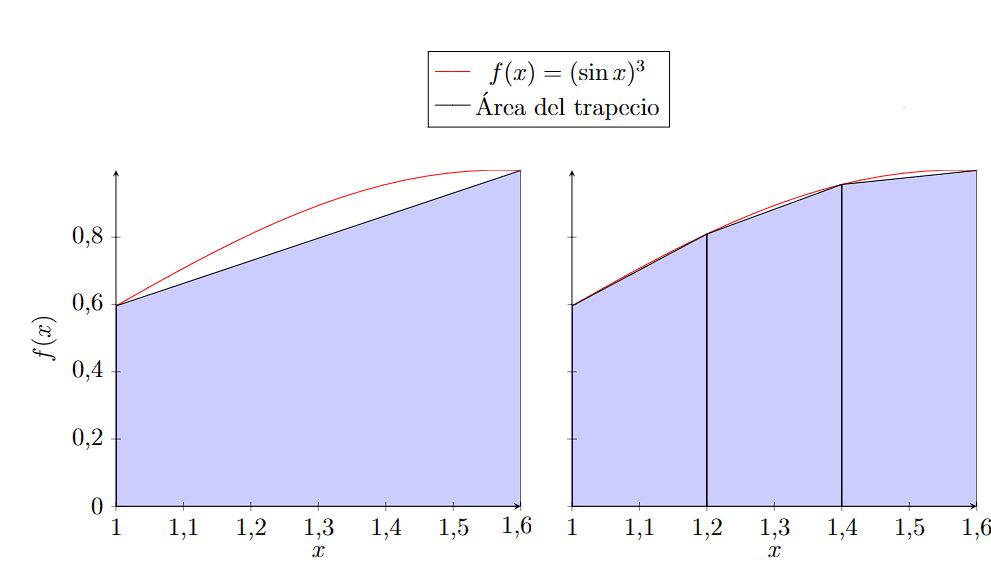
\includegraphics{fotos/trapecios.png}
    \end{adjustbox}
    \caption{En el lado izquierdo la regla del trapecio simple. A la derecha la regla del trapecio compuesta sobre tres intervalos (cuatro puntos).}
    \label{trap}
\end{figure}

Como podemos observar de esta manera nuestra aproximación del área es mucho más precisa solamente dividiendo en 3 intervalos.

\newpage
\begin{proof}

Si dividimos $[a,b]$ en $n$ subintervalos definidos por los $n + 1$ puntos:
$a =x_0 <x_1 <\cdots < x_{n-1} < x_n = b$ , $h = \frac{b-a}{n}$, tenemos:
\[
\int_{a}^{b} f (x)dx = \sum_{k=1}^{n} \int_{x_{k-1}}^{x_k} f (x)dx
\]
En cada intervalo $[x_{k-1},x_k]$ se aplica la regla del trapecio simple:
\[
\int_{a}^{b} f (x)dx = \sum_{k=1}^{n} \left[\frac{f (x_{k-1}) + f (x_k)}{2}h - \frac{f''(\xi_k)}{12} (h)^3\right]
\]
\[
= T_n - \frac{f''(\xi)}{12} \sum_{k=1}^{n} (h)^3 = T_n - \frac{f''(\xi)}{12} n(h)^3
\]
Como $h = \frac{b-a}{n}$, entonces:
\[
\int_{a}^{b} f (x)dx = T_n - \frac{f''(\xi)(b -a)^3}{12n^2}
\]
\end{proof}


\subsubsection{Error de aproximación en la regla de trapecios}

Este método conlleva un error absoluto que podemos acotar gracias a la siguiente expresión:

$$
E_n = \left| \int_{a}^{b} f(x)dx  - T_n\right| \leq \frac{K_2(b-a)^3}{12n^2}= \frac{K_2(b-a)}{12}(h)^2 \sim O(h^2)
$$
donde:
$$
K_2 = \max_{x \in [a, b]} |f''(x)|
$$

La correspondiente demostración se obtiene simultáneamente con la propia del método:

\begin{proof}
\[
E = \left|\int_{a}^{b} f (x)dx -T_n\right| = \left|\frac{f''(\xi)(b -a)^3}{12n^2}\right| = \frac{(b-a)^3}{12n^2} |f''(\xi)| \leq \frac{K_2(b -a)^3}{12n^2} = \frac{K_2(b-a)}{12} (h)^2
\]
donde:
\[
K_2 = \max_{x\in[a,b]} |f''(x)| 
\]
\end{proof}


\subsection{Regla de Simpson}

Al igual que el anterior método, la \textbf{regla de Simpson} es un mecanismo de integración numérica basado en funciones de interpolación (polinomios generalmente) utilizado para aproximar el valor de diversas funciones de interés. Esta regla es el resultado de combinar la regla del punto medio y la regla de los trapecios en una sola que reduzca los errores locales de la aproximación.\\

La regla de Simpson aproxima el área calculada por la integral en el intervalo $[x_{j-1} , x_{j+1}]$ mediante una parábola que pasa por tres puntos. En concreto:

\begin{center}
$x_{j-1} \hspace{2.5mm},\hspace{2.5mm} x_{j} \hspace{2.5mm},\hspace{2.5mm} x_{j+1}$
\end{center}

Al tratarse de una parábola, usamos como función con integral conocida (función de interpolación), el polinomio de interpolación de Lagrange de orden 2.\\

\begin{figure}[H]
\centering
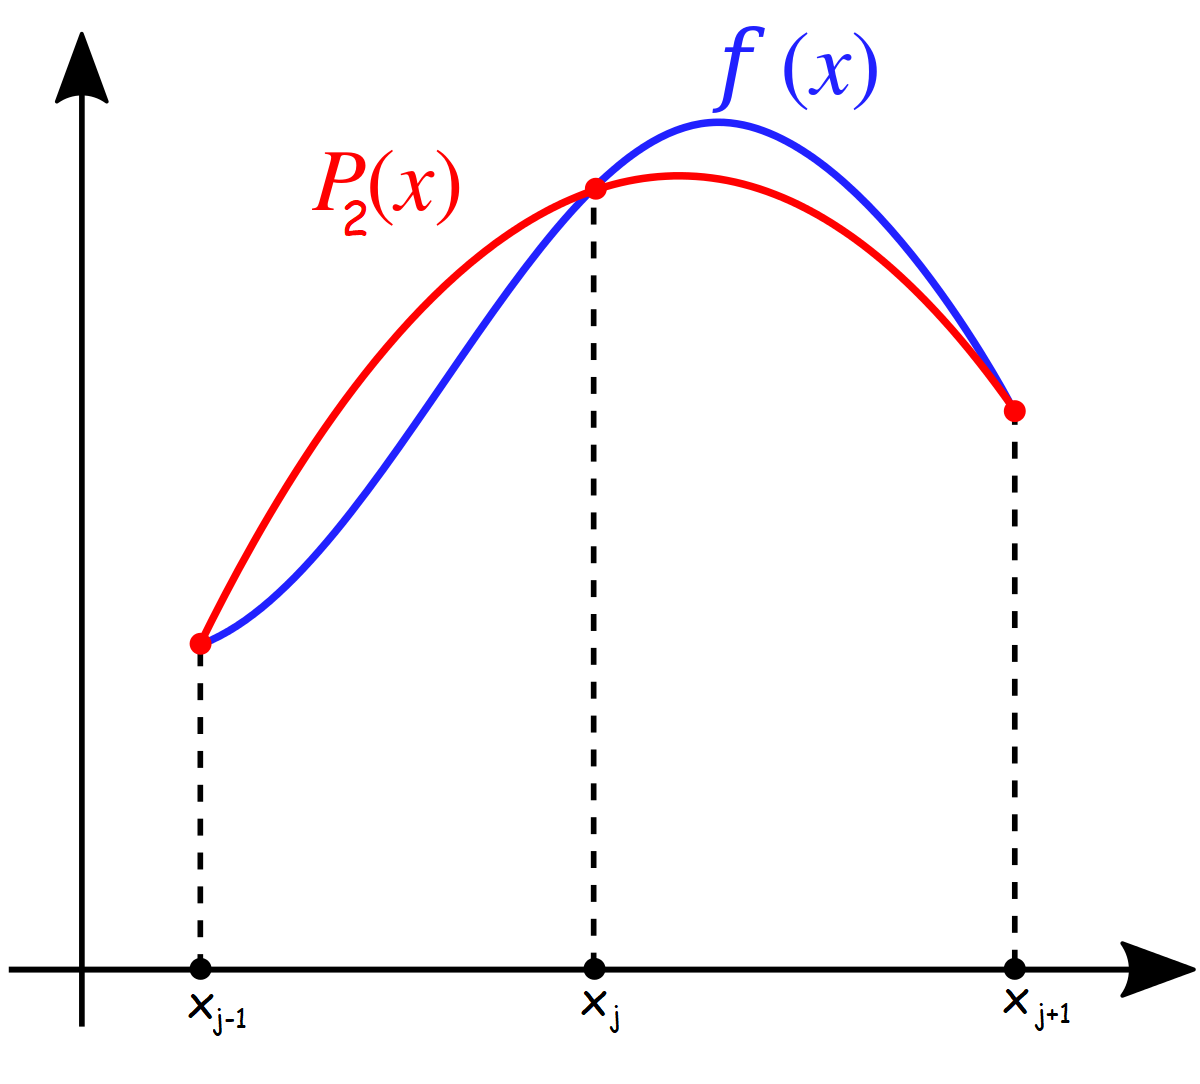
\includegraphics[scale=0.26]{intro}
\caption{Polinomio de Lagrange de orden 2 que pasa por tres puntos de la función que queremos aproximar.}
\end{figure}

Esta regla tiene dos desarrollos en función de la precisión que queramos obtener y en función del número de pasos a ejecutar. Son la regla de Simpson \textbf{simple} y la \textbf{compuesta}. Como el mayor interés de este trabajo es ver el método aplicado como parte de la resolución numérica, vamos directamente a hablar de la compuesta que es la que se utiliza a efectos prácticos.

\subsubsection{Regla de Simpson compuesta}

Esta regla no es más que la extensión de la regla simple para una región que no necesariamente sea el origen. Si queremos aplicarla a una función que se extiende por el plano, el primer paso es dividir la parte del dominio de la función que queramos aproximar en un número par \textbf{n} de intervalos. Es decir, hay que dividir el intervalo $[a,b]$ en n subintervalos donde n es un número par. Esto es:

\begin{center}
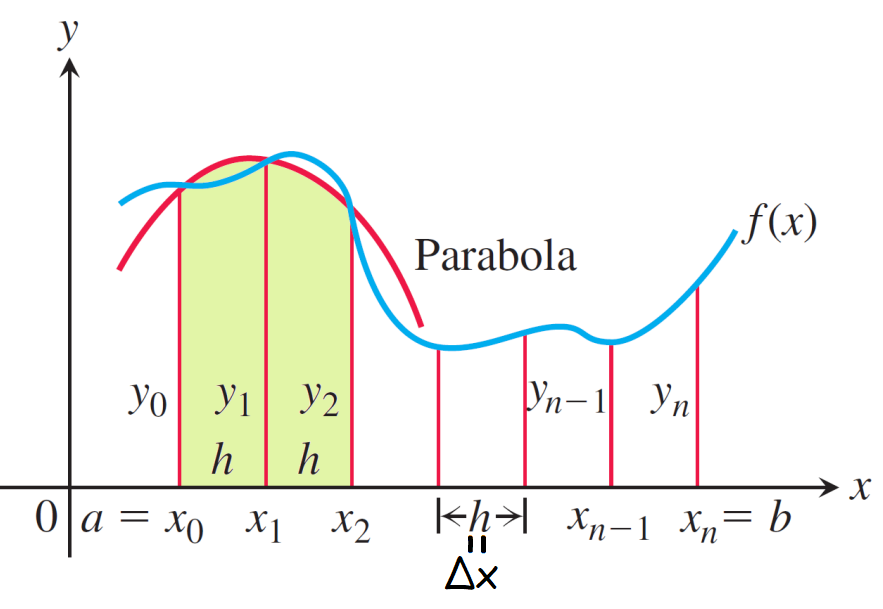
\includegraphics[width=0.6\linewidth]{simple_n}
\end{center}

Así, podemos escribir lo siguiente:

\begin{flushleft}
-Las posiciones $x_k$ corresponden a $x_k=a+h$ con $k=0,1,...,n$.\newline
-La anchura del intervalo, que denominamos paso, es $h=\frac{b-a}{n}$ .
\end{flushleft}

Con estas aclaraciones y la nueva notación, podemos escribir la expresión:

\begin{equation}
\int \limits_{x_{k-1}}^{x_{k+1}} f(x) \cdot dx \approx 
A(P_k) =
\frac{h}{3}(f(x_{k-1})+4f(x_k)+f(x_{k+1}))
\end{equation}

Ahora, debemos observar que como n es par, es decir, $n=2r$, ¡en nuestra aproximación vamos a tener r parábolas!\\

Con estas últimas consideraciones llegamos a la versión compuesta de este método. Básicamente consiste en aplicar la forma general de la versión simple de la regla sucesivas veces hasta cubrir la región finita que queramos aproximar.\\

Esto es lo que acabamos de ver, si dividimos el intervalo finito $[a,b]$ de la función en un número par \textbf{n=2r} de subintervalos de longitud $h=\frac{b-a}{n}$, llegamos a la siguiente expresión:
\begin{equation*}
\int \limits_{a}^{b} f(x) \cdot dx \approx 
 \sum_{k=1}^{r}A(P_k) =
\frac{h}{3}\sum_{k=1}^{r}[f(x_{2k-2})+4f(x_{2k-1})+f(x_{2k})] =
\end{equation*}
\begin{equation*}
\;\;\;\;\;\;\;\;\;\;\;\;
=\frac{h}{3}[f(x_0)+4\sum_{k=1}^{r}f(x_{2k-1})+2\sum_{k=1}^{r-1}f(x_{2k})+f(x_n)] =
\end{equation*}
\begin{equation}
\;\;\;\;\;\;\;\;\;
=\frac{h}{3}[f(a)+4\sum_{k=1}^{r}f(x_{2k-1})+2\sum_{k=1}^{r-1}f(x_{2k})+f(b)]
\end{equation}

\subsubsection{Error de aproximación en la regla de Simpson}

En este método también podemos establecer una cota superior para el error cometido al aproximar la integral deseada. Para ello, definamos primero el error global en la etapa n.

\begin{equation}
E_n=\left |\displaystyle \int \limits_{a}^{b} f(x) \cdot dx - Sn\right |
\end{equation}

Ahora, sea $S_n$ el resultado de aplicar la regla de Simpson compuesta:
\begin{equation}
S_n = S_{2r} = \frac{h}{3}
[f(a)+4\sum_{k=1}^{r}f(x_{2k-1})+2\sum_{k=1}^{r-1}f(x_{2k})+f(b)]
\end{equation}

Y sea $K_4 = \smash{\displaystyle\max_{x \in [a,b]}} |f^{(4)}(x)|$. Entonces el error absoluto está acotado por:

\begin{equation}
E_n \leq \frac{K_4(b-a)^5}{180n^4} = \frac{K_4(b-a)}{180}(h)^4 \sim O(h^4)
\end{equation}

Obtenemos como resultado que la magnitud del error es del orden del paso que utilizamos a la cuarta ($O(h^4)$). Esto quiere decir, que si $f(x)$ es un polinomio de grado 3 o inferior, ¡la regla de Simpson es exacta!\\

\underline{\textbf{Nota}} \\

El método que acabamos de explicar también es conocido como la regla de Simpson 1/3. Existe otra variante de la regla que es la regla de Simpson 3/8, que difiere de la clásica en que esta usa polinomios de interpolación de Lagrange de 3er orden, además de que la función se tabula con cuatro puntos a igual distancia h formando tres subintervalos. \\

La regla 3/8, comparada en el mismo intervalo que la 1/3, es 2.25 veces más precisa que su compañera. Aún así, en la práctica, rara vez usamos el método 3/8 debido a que el aumento de complejidad es notable (n pasa a tener que ser múltiplo de tres, necesitamos polinomios de grado 3, etc) y debido a que en la mayoría de aplicaciones el método 1/3 nos proporciona la precisión suficiente.\\ 

\newpage
\section{Soluciones de la Ecuación de Schrödinger}
En esta sección del trabajo nos dedicaremos a obtener las soluciones de la ecuación de Schrödinger de forma numérica y compararlas con las soluciones analíticas de la misma en regiones del espacio donde existen potenciales distintos.

\subsection{Pozo de potencial infinito}

En este primer caso nos encontramos en una región del espacio cubierta por un potencial infinito en toda ella menos en un intervalo finito donde ese potencial tiene un valor de 0, como podemos observar en la siguiente figura:

\begin{figure}[H]
    \centering
    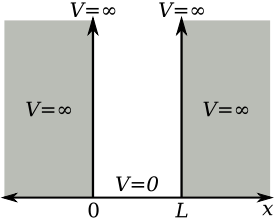
\includegraphics[width=0.5\linewidth]{fotos/particula-caja-wiki.png}
    \caption{Pozo de potencial infinito}
\end{figure}

Una vez planteado el escenario, veamos las funciones de onda que describen a las partículas que nos podemos encontrar aquí y sus niveles de energía correspondientes.

    \subsubsection{Soluciones analíticas}
    Empecemos por hallar sus soluciones analíticas, es decir, las soluciones que obtendríamos si introducimos nuestro potencial junto con el Hamiltoniano en la ecuación de Schrödinger y resolvemos el problema de autovalores y autofunciones bajo esas condiciones.\\

    La solución la podemos escribir según la posición de nuestra partícula:

    \begin{itemize}
        \item \underline{Para x$<$0 y x$>$L}\\
        La función de onda deber ser nula pues para estar en esta región del espacio una partícula necesitaría energía infinita. Por tanto:

        \begin{equation*}
            \psi (x) = 0
        \end{equation*}

        \item \underline{Para 0$<$x$<$L}\\
        Para satisfacer las condiciones de contorno, la función también debe anularse en los extremos del intervalo, esto es:
        
        \begin{equation*}
            \psi (0) = \psi (L) = 0
        \end{equation*}
    
    Con esto definido, en esta región la ecuación de Schrödinger toma la forma: 

    \begin{equation}
    \frac{d^{2}\psi(x)}{d x^{2}} = -\frac{2m}{\hbar^2} E \psi(x)
    \end{equation}

    Por lo que ante este problema de Sturm-Liouville se propone la solución correspondiente para resolverlo. El resultado final y por tanto la forma de nuestras soluciones analíticas para cada nivel discreto de energía es:

\begin{equation*}
    \boxed{\psi_n (x) = A\cdot\sin{\left(\frac{n\pi}{a}x\right)}\,\,\,\,\,\,\,\,\,\,\,\, n=1,2,3,...}
\end{equation*}

    donde A es una constante de normalización de valor $A=\sqrt{\frac{2}{a}}$ y $a$ es el límite inferior que delimita el pozo.\\

    Además, los mencionados niveles discretos de energía, que son los autovalores correspondientes a cada autofunción obtenida son los siguientes:

    \begin{equation*}
    \boxed{E_n = \frac{\hbar^2n^2\pi^2}{2ma^2}\,\,\,\,\,\,\,\,\,\,\,\, n=1,2,3,...}
    \end{equation*}

    \end{itemize}

    \subsubsection{Soluciones numéricas}

    El método de obtención de las soluciones numéricas es análogo para las soluciones que siguen. Consiste en realizar una discretización del espacio gracias al método de diferencias finitas y construir el problema de autovalores de forma matricial. Cada solución lleva consigo su propio potencial, lo que modificará la matriz H del Hamiltoniano.\\

    Los autovalores y las autofunciones de esta matriz son las soluciones aproximadas que estamos buscando. Los valores de las autofunciones pueden no estar normalizados, condición necesaria para que lo que estamos estudiando tenga un significado físico, aquí es donde entran los métodos numéricos de integración.\\

    Para normalizar nuestras funciones usaremos tanto el método de los trapecios como el método de Simpson. Con estas funciones ya podremos comparar nuestras soluciones numéricas (aproximadas) con las soluciones analíticas que hemos descrito. La diferencia entre ambas se corresponderá con el error en la aproximación y en la siguiente sección trataremos este tema con detalle.\\
    
    Primero visualicemos lo que hemos explicado para cada solución estudiada en este trabajo. Empecemos por el pozo de potencial infinito, indicando las condiciones que utilizamos para realizar las siguientes representaciones:\\

     El potencial V(x)=0 existe en la región del espacio delimitada por los límites a=0 y b=5. Ese es nuestro intervalo de trabajo. Para hacer la aproximación cogemos un N=1000 puntos y representamos 5 funciones de onda.\\

     Además, con el objetivo de simplificar los cálculos, se han utilizado los siguientes valores para la constante de Planck reducida $\hbar=1$ y la masa $m=1$.\\
     
     Los resultados han sido los siguientes:\\

     \textit{Nota: Para mejorar la visualización del gráfico, a cada función de onda se le ha sumado dos veces su nivel de energía para que las ondas aparecieran separadas sin superponerse.}

     \begin{figure}[H]
         \centering
         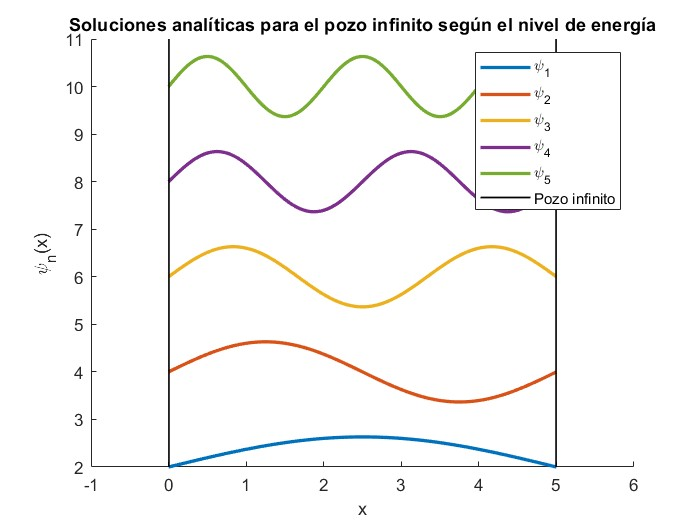
\includegraphics[width=0.9\linewidth]{fotos/infinito_analiticas.jpg}
         \caption{Funciones analíticas según el nivel de energía. En el eje horizontal representamos la región del espacio y en el vertical la función de onda más dos veces su nivel de energía (2$\cdot$n con n=1,2,3,4,5).}
     \end{figure}

     \begin{figure}[H]
         \centering
         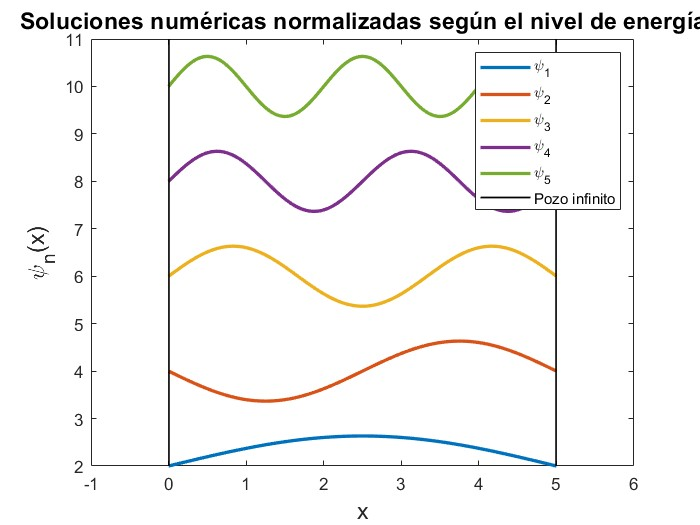
\includegraphics[width=0.9\linewidth]{fotos/infinito_numericas.jpg}
         \caption{Funciones aproximadas por métodos numéricos según el nivel de energía. En el eje horizontal representamos la región del espacio y en el vertical la función de onda más dos veces su nivel de energía (2$\cdot$n con n=1,2,3,4,5).}
     \end{figure}
     \vspace{5mm}
En este punto y en los que siguen hay una pequeña aclaración que hay que comentar. Como hemos explicado, nosotros procedemos primero discretizando el espacio con diferencias finitas y después diagonalizando la matriz del Hamiltoniano. De esta última sacamos los autovalores y las autofunciones con la función \textit{eig()} de MATLAB. Si recordamos algo de álgebra lineal, para un mismo autovalor, hay dos vectores propios asociados, la autofunción y su inversa (la misma autofunción pero multiplicada por -1).\\

Esto no nos influye a la hora de calcular los errores de aproximación, pero sí se observa en las gráficas, por lo que hay que tenerlo en cuenta. Para ejemplificar lo que estamos explicando mostremos dos niveles de energía de las autofunciones del pozo infinito en la siguiente figura:




\begin{figure}[H]
    \centering
    \begin{adjustbox}{width=1.1\linewidth,center}
        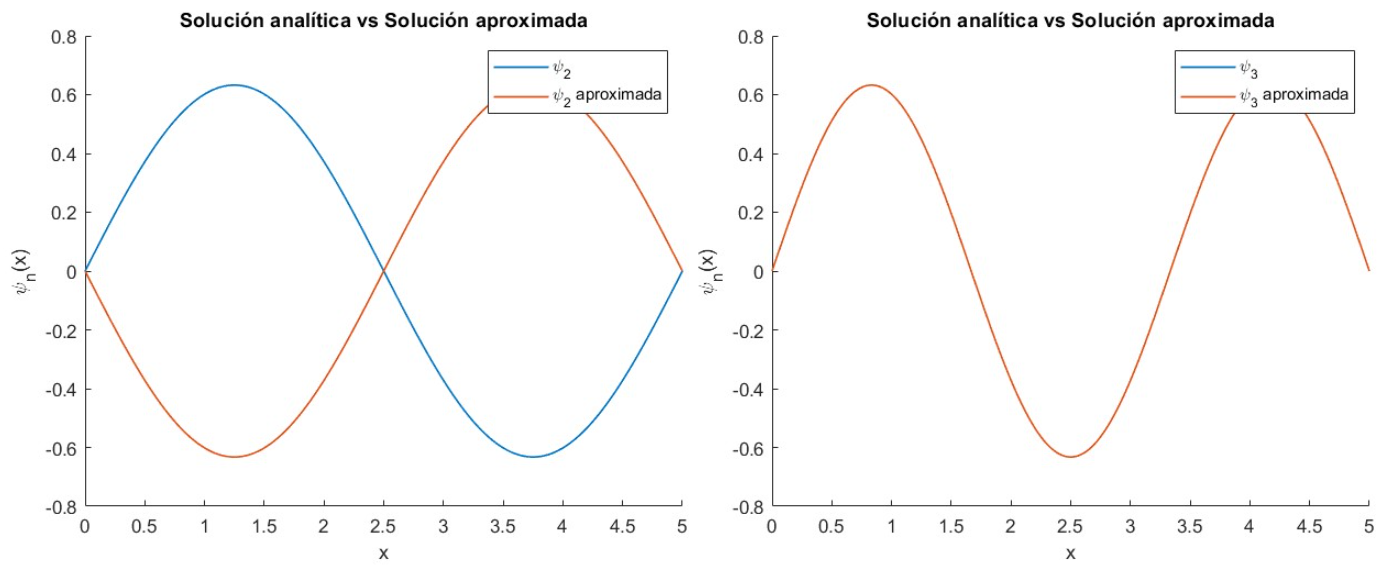
\includegraphics{fotos/autofunciones_invertidas.png}
    \end{adjustbox}
    \caption{A la izquierda una autofunción que resulta invertida respecto a la solución analítica. En el lado derecho, ambas funciones, numérica y analítica coinciden en signo.}
\end{figure}

Tras mostrar las funciones de onda, hacemos lo propio para los niveles de energía obtenidos numérica y analíticamente.

\begin{figure}[H]
    \centering
    \begin{adjustbox}{width=1.2\linewidth,center}
        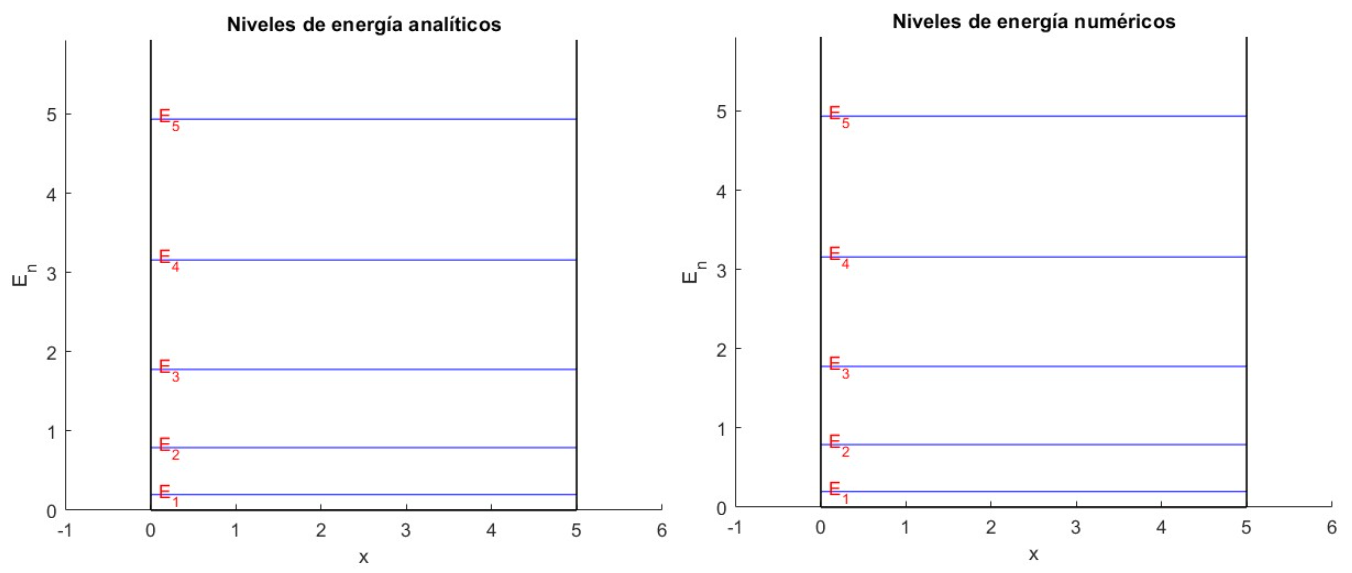
\includegraphics{fotos/comp_energias_infinito.png}
    \end{adjustbox}
    \caption{A la izquierda niveles de energía analíticos representados a modo de esquema en la misma región que el pozo. A la derecha, niveles de energía obtenidos por métodos numéricos. Los niveles corresponden a n=1,2,3,4 y 5.}
\end{figure}

\newpage
Los valores obtenidos tanto analítica como numéricamente se recogen en la siguiente tabla:

\begin{table}[H]
    \centering
    \begin{tabular}{|c||c||c|}
    \hline
        $E_n$ & Valor analítico & Valor numérico \\ \hline \hline
        $E_1$ & 0.197392088021787 & 0.197391925353448 \\ \hline
        $E_2$ & 0.789568352087149 & 0.789565749317132 \\ \hline
        $E_3$ & 1.776528792196085 & 1.776515615673212 \\ \hline
        $E_4$ & 3.158273408348594 & 3.158231764114112 \\ \hline
        $E_5$ & 4.934802200544679 & 4.934700530344333 \\ \hline
    \end{tabular}
    \caption{Datos obtenidos de la simulación para las energías de cada función de onda. Estos datos representan los autovalores correspondientes a cada autofunción.}
\end{table}

Con esto tenemos a disposición los resultados necesarios para ver que los procedimientos han sido correctos y que la aproximación, en primera instancia, es bastante aceptable dentro de los parámetros de la simulación. Queda pendiente el análisis de los errores que se realizará en la sección~\ref{sec:errores} de este trabajo.

        \subsection{Oscilador armónico cuántico}

    El oscilador armónico tiene una gran importancia en la física 
    y se utiliza en una amplia gama de campos debido a su capacidad para modelar una variedad de fenómenos naturales.\\
    
    Clásicamente, un oscilador armónico se describe por la posición $x(t)$ de una partícula de masa m y su momento $p(t)$. La energía $E$ de una partícula con posición y momento viene dada por $E = \frac{p^2}{2m} + \frac{1}{2}m\omega^2x^2$.
    Donde $\omega$ es la frecuencia angular del sistema y viene dada por $\omega=\frac{2\pi}{T}$ y $T$ es el periodo de oscilación del sistema.\\
    
    Para este caso también se cumple que $\omega=\sqrt{\frac{k}{m}}$ ya que la partícula de masa $m$ siente una fuerza de atracción dada por $F=-kx$, siendo $k$ la constante elástica.\\
    
    El problema con este oscilador clásico es que no podemos usarlo para describir sistemas donde los efectos cuánticos sean considerables. Para solucionar esto convertimos nuestro momento y posición en los operadores hermíticos $\hat{x}$ y $\hat{p}$. Con estos construimos nuestro Hamiltoniano que, inspirado en la energía clásica, queda:
    
    \begin{equation}
    \hat H\equiv \frac{\hat{p}^2}{2m} + \frac{1}{2}m\omega^2\hat{x}^2
    \end{equation}

    \subsubsection{Soluciones analíticas}
    Según lo que acabamos de explicar, la ecuación de Schrödinger independiente del tiempo para este Hamiltoniano toma la siguiente forma:
    
    \begin{equation}
        \frac{-\hbar^2}{2m}\frac{\partial^2\psi(x)}{\partial x^2} + \frac{1}{2}m\omega^2x^2\psi(x)=E\psi(x)
    \end{equation}
    
    Esta ecuación tiene como solución analítica las funciones de onda ya normalizadas:
    
    \begin{equation}
        \boxed{\psi _n\left(x\right)=\frac{1}{\sqrt[2]{2^n\cdot \:n!}\cdot \pi ^{\frac{1}{4}}}\cdot \:H_n\left(x\right)e^{-\frac{x^2}{2}}}
    \end{equation}
    
    Siendo los $H_n$ los correspondientes polinomios de Hermite, que son polinomios ortogonales con la siguiente forma:
    
    \begin{figure}[H]
        \centering
        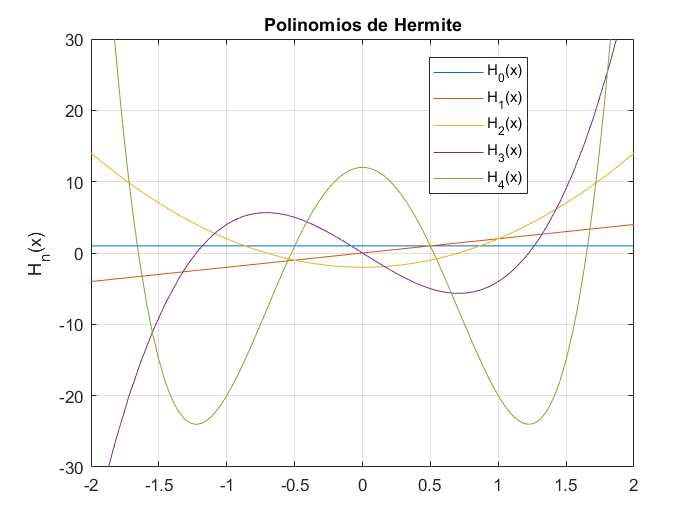
\includegraphics[width=0.75\textwidth]{fotos/PolinomiosHermite.png}
        \caption{Cuatro primeros polinomios de Hermite.}
        \label{PolinomiosHermite}
    \end{figure}
    
    Con energías asociadas de la forma:
    
    \begin{equation}
        \boxed{E_n=\left(n+\frac{1}{2}\right)\hbar \omega }
    \end{equation}

    \subsubsection{Soluciones numéricas}
    
    Para nuestras soluciones numéricas usaremos la frecuencia del oscilador $\omega=1$ la constante de Planck reducida $\hbar=1$ y la masa $m=1$ con el objetivo de facilitar los cálculos.\\
    
    Definimos nuestro potencial como $V(x)=\frac{1}{2}m\omega^2x^2$ y trabajamos en el intervalo [-8,8] dividido en 1000 puntos, ya que con estos parámetros nuestra solución es lo suficientemente precisa y no lleva un tiempo de computación excesivamente largo.\\

    \newpage
    De nuestro método de diferencias finitas obtenemos las siguientes energías:\\
    
        \begin{table}[H]
            \centering
            \begin{tabular}{|c||c||c|}
            \hline
             $E_n$& Solución Numérica &Solución Analítica \\ [0.5ex] 
            \hline\hline
            $E_0$& 0.499991 & 0.500000 \\
            \hline
            $E_1$& 1.499959 & 1.500000 \\
            \hline
            $E_2$& 2.499895 &  2.500000\\
            \hline
            $E_3$& 3.499800  & 3.500000 \\
            \hline
            $E_4$& 4.499671 & 4.500000\\
            \hline
            $E_5$& 5.499511 & 5.500000 \\
            \hline
            $E_6$& 6.499319 & 6.500000 \\
            \hline
            $E_7$& 7.499094  & 7.500000 \\
            \hline
            $E_8$& 8.498838 & 8.500000 \\
            \hline
            $E_9$& 9.498549 & 9.500000 \\
            \hline
            $E_{10}$& 10.498228 & 10.500000 \\
            \hline
             $E_{11}$& 11.497875& 11.500000 \\
            \hline
            $E_{12}$& 12.497490 & 12.500000 \\
            \hline
            $E_{13}$& 13.497075 & 13.500000 \\
            \hline
            $E_{14}$& 14.496624 & 14.500000 \\
            \hline
            $E_{15}$& 15.496143 & 15.500000 \\
            \hline
            \end{tabular}
            \caption{Tabla de soluciones de energías del OAC.}
            \end{table}
            
    Se puede apreciar un ligero error de nuestras soluciones. Esto es debido al error propio del método de diferencias finitas, ya que nuestro paso en este caso era de $h=0.16$.\\
    
    Ahora mostraremos nuestros autovectores obtenidos de manera numérica, pero es importante resaltar que estos acumulan el error de diferencias finitas y del método que usemos para la normalización de estos. En este caso usaremos Simpson porque es el que menos error presenta.
    
    \begin{figure}[H]
        \centering
        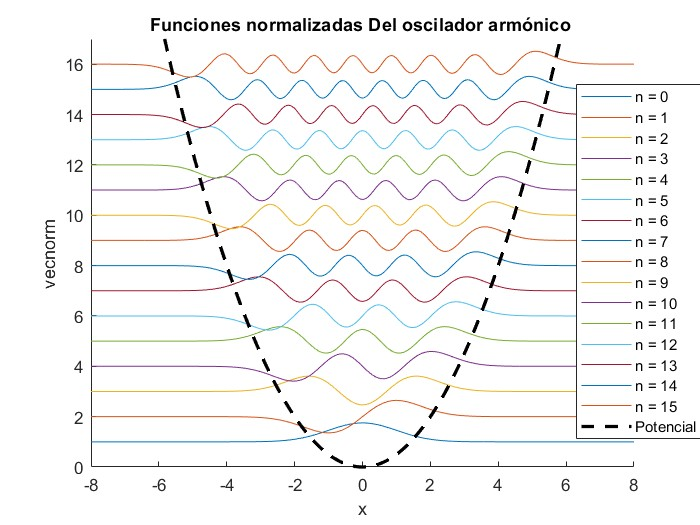
\includegraphics[width=0.9\textwidth]{fotos/16funcionesoscilador.jpg}
        \caption{Se muestran los 16 vectores normalizados.}
    \end{figure}
    
    Aquí cada nivel lo hemos separado sumando a cada función su nivel de energía más uno para que fuese más legible pero realmente todas tienden a 0 en los extremos y están normalizadas.\\
    
    Además nuestro código de diferencias finitas nos devolvía los vectores con un desfase de $\pi$ como ya fue expuesto en el pozo infinito así que también hubo que ajustarlo. \\
    
    Si nos acercamos al punto marcado podemos ver que nuestra función para el nivel 15 no es exactamente igual que la solución analítica pero es un error muy pequeño como para que podamos apreciarlo. Este punto es uno de los que más difiere puesto que a mayor nivel de energía más error nos encontramos. Esto también era visible en los errores de energía, a mayor error en la autovector mayor error en su autovalor asociado.
    
    \begin{figure}[H]
        \centering
        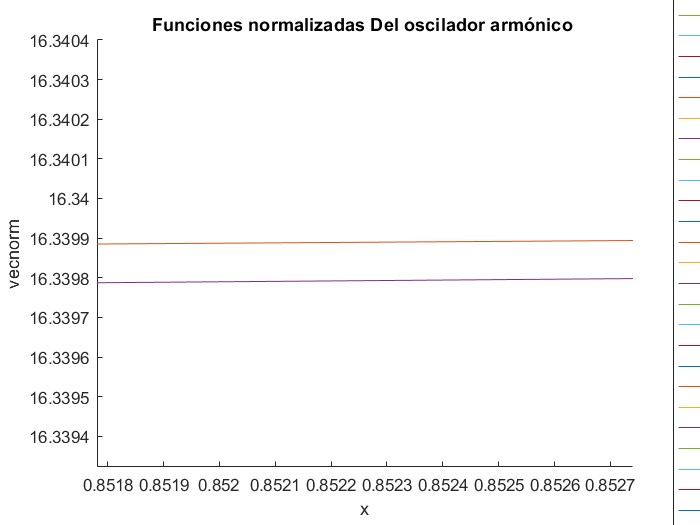
\includegraphics[width=0.8\textwidth]{fotos/diferenciaentrefunciones.jpg}
        \caption{Zona ampliada de la función con n=15 (punto marcado) donde se aprecia la diferencia entre la solución numérica y la analítica.}
    \end{figure}

    \subsection{Pozo de potencial finito}
    
    \subsubsection{Soluciones analíticas}
    
    \textbf{\underline{Características principales}}\\
    
Un pozo de potencial finito es una de las estructuras básicas utilizadas en física cuántica para observar el comportamiento de la función de onda de una partícula. Este pozo viene descrito por el siguiente potencial:

\begin{equation*}
V(x)=\begin{cases} 
    0 & \text{si} \quad -\infty < x \leq -a \\
    -V_0 & \text{si} \quad -a\leq x \leq a \\
    0 & \text{si} \quad a \leq x < \infty \\
 \end{cases}
\end{equation*}

Siendo $V_0$ positivo.\\

Si resolvemos la ecuación de autovalores del Hamiltoniano vamos
a obtener diferentes soluciones en función del tramo en el que 
nos encontremos y dependiendo de si la función es par o impar. Por simplicidad,
vamos a clasificarlas en función de si la solución es par o impar: \\

Si la solución es par obtenemos:

\begin{equation}
    \boxed{\psi^{(+)}(x)=\begin{cases} 
        C e^{\beta x} & \text{si} \quad -\infty < x \leq -a \\
        A\cos(\alpha x) & \text{si} \quad -a\leq x \leq a \\
        C e^{-\beta x} & \text{si} \quad a \leq x < \infty \\
     \end{cases}}
\end{equation}

Por otra parte, si la solución es impar tendremos:

\begin{equation}
    \boxed{\psi^{(-)}(x)=\begin{cases} 
        -C e^{\beta x} & \text{si} \quad -\infty < x \leq -a \\
        B\sin(\alpha x) & \text{si} \quad -a\leq x \leq a \\
        C e^{-\beta x} & \text{si} \quad a \leq x < \infty \\
     \end{cases}}
\end{equation}

Donde A, B y C son las constantes de normalización y $\alpha$ y $\beta$ vienen definidos como: 

\begin{center}
    $\alpha=\frac{\sqrt{2m(\left\lvert V_0 \right\rvert-\left\lvert E \right\rvert)}}{\hbar}$
\hspace{0.3cm};\hspace{0.3cm} $\beta=\frac{\sqrt{2m\left\lvert E \right\rvert}}{\hbar}$ 
\end{center}

Como vemos, las constantes de normalización dependen de los  valores de la energía y de $V_0$. Es decir, variarán según cómo se haya construido el pozo. En la siguiente sección hablaremos sobre el pozo que vamos a analizar y el valor de las constantes de normalización.

\begin{figure}[H]
    \centering
    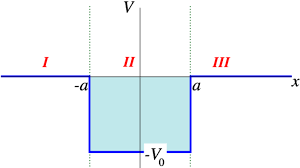
\includegraphics[width=0.7\linewidth]{images.png}
    \caption{Pozo de potencial finito}
\end{figure}

\subsubsection{Construcción del pozo de potencial}
Para este pozo se ha usado el valor para la profundida del pozo
de: $V_0=50$ (unidades arbitrarias). Además, como en el ordenador
no podemos incluir el infitio como en la definición formal, hemos 
decidido usar como aproximación en los extremos de análisis $\pm 8$ ya
que, como veremos más adelante, con poner estos intervalos como
aproximación es suficiente para ver sin problemas el comportamiento
de las funciones de onda para este potencial. Por último, hemos decidido situar el pozo en la región de -5 a 5.\\

Teniendo todo esto en cuenta, hemos obtenido las siguientes constantes de normalización: $A=B=0,44$ y $C=6.1\cdot 10^{14}$. Para ello, hemos usado la definición de normalización:

\begin{equation}
\int_{a}^{b} \psi^{*}(x) \psi(x) \,dx=1
\end{equation}

Un apunte importante es que para todos los cálculos se ha considerado que $\hbar~=~m~=~1$. \\

A continuación, en la siguiente sección mostraremos las soluciones numéricas y las compararemos con las obtenidas analíticamente.

\subsubsection{Soluciones numéricas}

Las soluciones numéricas han sido obtenidas para un número de puntos N=1000 y un total de 5 funciones. Las soluciones analíticas
para esas funciones son: 

\begin{figure}[H]
    \centering
    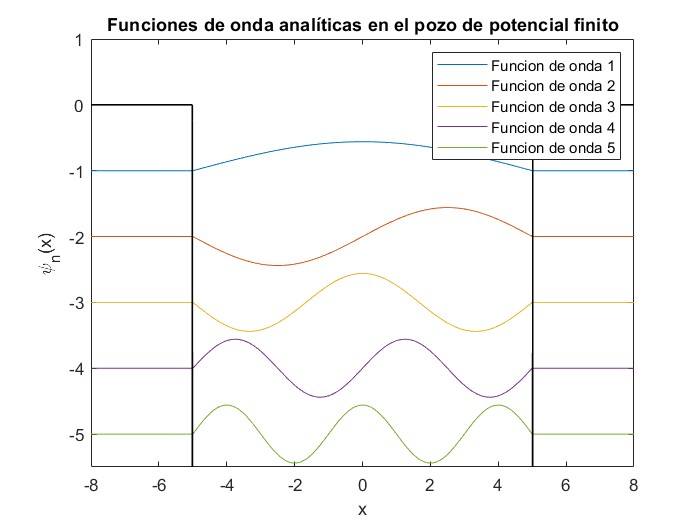
\includegraphics[width=1.0\textwidth]{analiticas.jpg}
    \caption{Primeras 5 soluciones analíticas del pozo de potencial finito}
\end{figure}

\newpage
Mientras que las soluciones numéricas son las siguientes:

\begin{figure}[H]
    \centering
    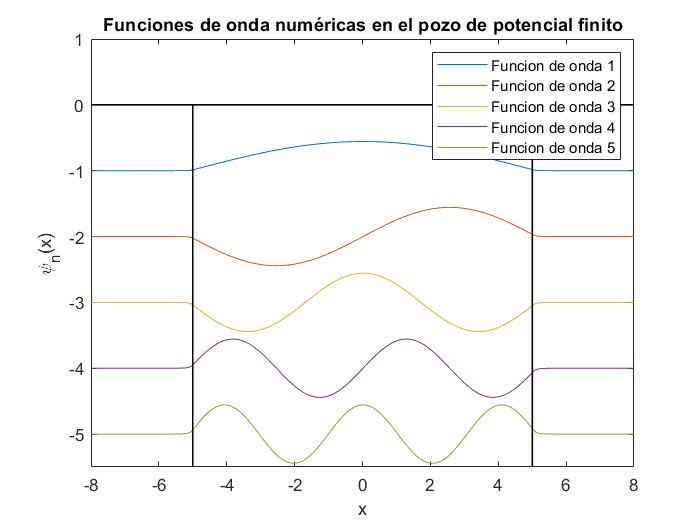
\includegraphics[width=1.0\textwidth]{numericas.jpg}
    \caption{Primeras 5 soluciones numéricas del pozo de potencial finito}
\end{figure} 
Como es fácilmente observable, las aproximaciones numéricas
son bastante aceptables. Algo que confirmaremos en el tratamiento
de errores. \\
\par 
Además, hemos equiespaciado dentro del pozo las funciones de onda
por dos motivos: el primero es que es más sencilla la visualización
de todas las ondas de este modo; y el segundo es debido a que,
como veremos a continuación, la energía que transporta esta 
función de onda es negativa. Esto quiere decir que estamos 
estudiando estados ligados y, por tanto, la mejor manera para 
visualizar estos estados es con las funciones de onda dentro del
pozo, no por encima de él. \\

Con esta aclaración hecha, vamos a proceder a enseñar las 
energías analíticas y numéricas con su respectiva tabla de 
errores:

\begin{figure}[H]
    \centering
    \begin{adjustbox}{width=1.2\linewidth,center}
        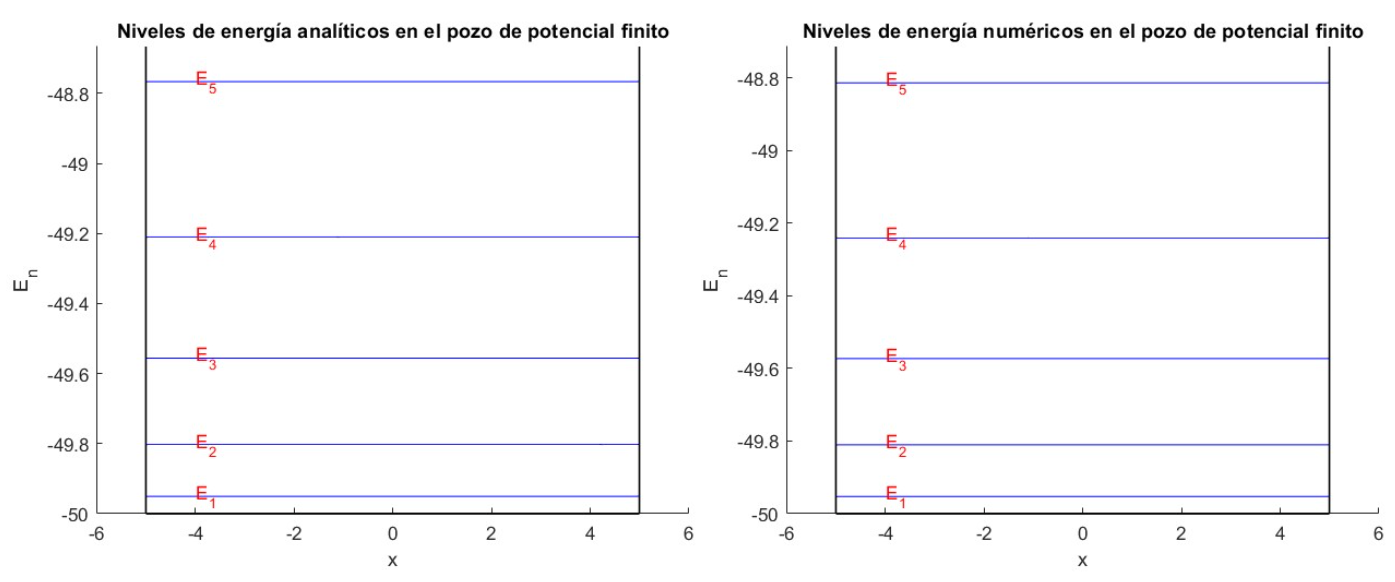
\includegraphics{fotos/comp_energias_finito.png}
    \end{adjustbox}
    \caption{A la izquierda niveles de energía analíticos representados a modo de esquema en la misma región que el pozo. A la derecha, niveles de energía obtenidos por métodos numéricos. Los niveles corresponden a n=1,2,3,4 y 5.}
\end{figure}

La tabla de errores nos arroja los siguientes resultados:
\begin{table}[H]
    \centering
    \begin{tabular}{|c||c||c|}
    \hline
    Nivel de energía($E_n$) & Energía analítica & Energía numérica \\
    \hline \hline 
    1 & -49,95065198 & -49,95251866  \\
    \hline
    2 & -49,80260791 & -49,81007930  \\
    \hline
    3 & -49,5558678 & -49,57269590   \\
    \hline
    4 & -49,21043165 & -49,24039191  \\
    \hline
    5 & -48,76629945 & -48,81320046  \\
    \hline
    \end{tabular}
    \caption{Energías del pozo de potencial finito.}
 \end{table}
 
Vemos que, según la energía va siendo mayor, el error se hace 
cada vez más grande. El principal motivo es que las energías analíticas se obtienen a partir de una aproximación la cual es:

\begin{equation*}
    \boxed{E_n\approx V_o+\frac{n^2\hbar^2\pi^2}{8ma^2}}
\end{equation*}

Con lo cual, esto provoca que la discrepancia entre resultados sea mayor. Sin embargo, debido a que el orden de error es bastante bajo, podemos dar como válidas nuestras soluciones numéricas.

\newpage
\section{Estudio de errores para las soluciones obtenidas}
\label{sec:errores}

En esta sección vamos a centrarnos en estudiar los errores que cometemos a la hora de aproximar las soluciones, es decir, trataremos de ilustrar el error que tienen asociados los métodos numéricos que hemos empleado para obtener los resultados que hemos mostrado en el trabajo.\\

Los parámetros de la simulación se indicarán en cada apartado pero el procedimiento será general para sendos. Primero calcularemos el error como describimos a continuación y lo representaremos en función del paso o del número de puntos dependiendo del apartado (un caso es análogo al otro). Posteriormente transformaremos esa gráfica a la misma pero tomando logaritmos en ambos miembros para una mejor visualización.\\ 

El método que vamos a seguir para estudiar el error será calcular la raíz del error cuadrático medio tanto de energías como de funciones para diferentes pasos. Teóricamente, según se reduce el paso, el error cometido también debe descender, para comprobar esto graficaremos nuestros resultados y veremos si cumplen esta tendencia. \\

La raíz del error cuadrático medio (RMSE) para las energías será:

\[
\text{RMSE} = \sqrt{\frac{1}{n} \sum_{i=1}^{n} (E_i - \hat{E}_i)^2}
\]

Donde:
\begin{itemize}
    \item \( n \) es el número de niveles.
    \item \( E_i \) es la energía analítica del nivel i.
    \item \( \hat{E}_i \) es la energía numérica del nivel i.
\end{itemize}

La raíz del error cuadrático medio (RMSE) para las autofunciones se calculara como:

\[
\text{RMSE} =\sqrt{\frac{1}{n}\sum_{i=1}^{n}\frac{1}{N} \sum_{k=1}^{N} (\psi_n(x_k) - \hat{\psi}_n(x_k))^2}
\]

Donde:
\begin{itemize}
    \item \( n \) es el número de niveles.
    \item \( \psi_i(k) \) es la autofunción analítica en el nivel i evaluada en el punto $x_k$.
    \item \( \hat{\psi}_i(k) \) son las autofunciones numéricas en el nivel i evaluada en el punto $x_k$.
    \item \( N \) es el número de puntos con los que se divide el intervalo.
\end{itemize}


    \subsection{Pozo de potencial infinito}

    \subsubsection{Error en las energías}

    A continuación se va a representar cómo varía el error en los niveles de energía en función del número de puntos que tomemos para realizar la discretización del espacio (cuantos más puntos, menor será el paso, por lo que se podría hacer un gráfico análogo del error en función del paso).\\
    
    Lo que acabamos de comentar significa que nuestros resultados pueden ser estudiados tanto en función del número de pasos como en función del tamaño del paso. Como prueba de ello este primer resultado, el del pozo infinito, vamos a representarlo en función de N y en el resto de casos, ya que lo creemos más oportuno, en función de h.\\ 

    Decimos que es más oportuno ya que el error asociado al tamaño del paso no varía con la longitud del intervalo, mientras que el asociado al número de puntos sí lo hace (nuestros errores van como potencias de $h$ y no de N).\\
    
    Para la simulación vamos a coger valores de N comprendidos entre 10 y 500.\\

\begin{figure}[H]
    \centering
    \begin{adjustbox}{width=1.2\linewidth,center}
        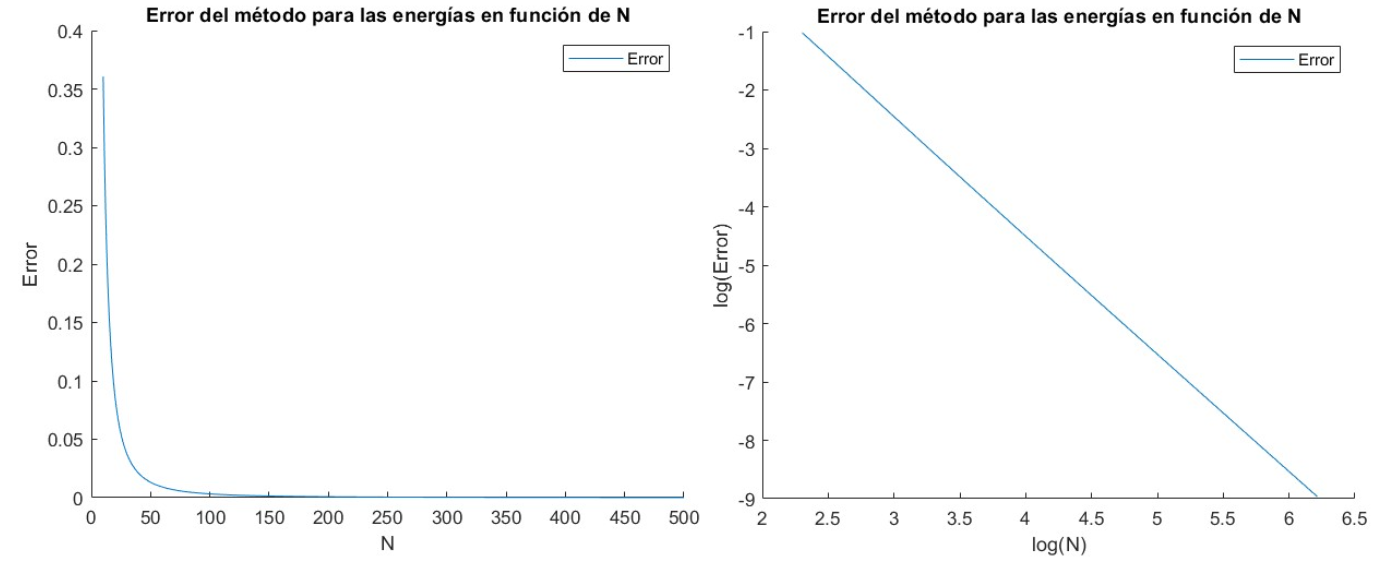
\includegraphics{fotos/comperror_energias_infinito.png}
    \end{adjustbox}
    \caption{A la izquierda la raíz del error cuadrático medio en las energías (Error), según el numero de puntos (N). A la derecha, el logaritmo de la raíz del error cuadrático medio en las energías (~log(Error)~), según el logaritmo del numero de puntos(~log(N)~).}
\end{figure}

\subsubsection{Error en las funciones}
Ahora se mostrará la evolución del error 
para las funciones según el número de puntos. 
Al igual que antes, N tomará valores desde 10 hasta 500.
La normalización de las funciones se ha hecho mediante 
el método de Simpson para la integración numérica.\\

    Cabe destacar que en esta ocasión se ha usado un gráfico de dispersión debido a las oscilaciones presentes en los valores de los datos. Para evitar llegar a conclusiones equivocadas se muestran los puntos y se relaciona con un ajuste conocido (logarítmico para el primer caso y lineal para el segundo).
    
   \begin{figure}[H]
    \centering
    \begin{adjustbox}{width=1.2\linewidth,center}
        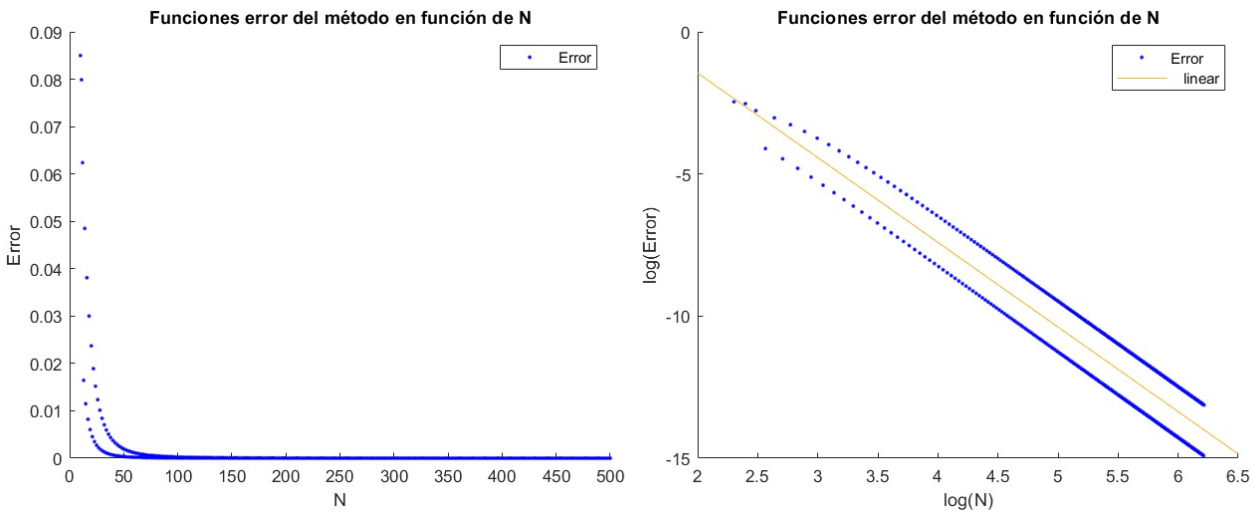
\includegraphics{fotos/comperror_funciones_infinito.png}
    \end{adjustbox}
    \caption{A la izquierda la raíz del error cuadrático medio en las funciones (Error), según el numero de puntos (N). A la derecha, el logaritmo de la raíz del error cuadrático medio en las funciones (~log(Error)~), según el logaritmo del numero de puntos(~log(N)~).}
\end{figure}
    
    \subsection{Oscilador armónico cuántico}

    \subsubsection{Error en las energías}

    A continuación mostraremos como evoluciona el error en las energías en función del paso que utilicemos en nuestros métodos de aproximación. Lo realizaremos viendo como varía el mismo si dividimos el espacio con N puntos donde N toma valores desde 20 hasta 500.

\begin{figure}[H]
    \centering
    \begin{adjustbox}{width=1.2\linewidth,center}
        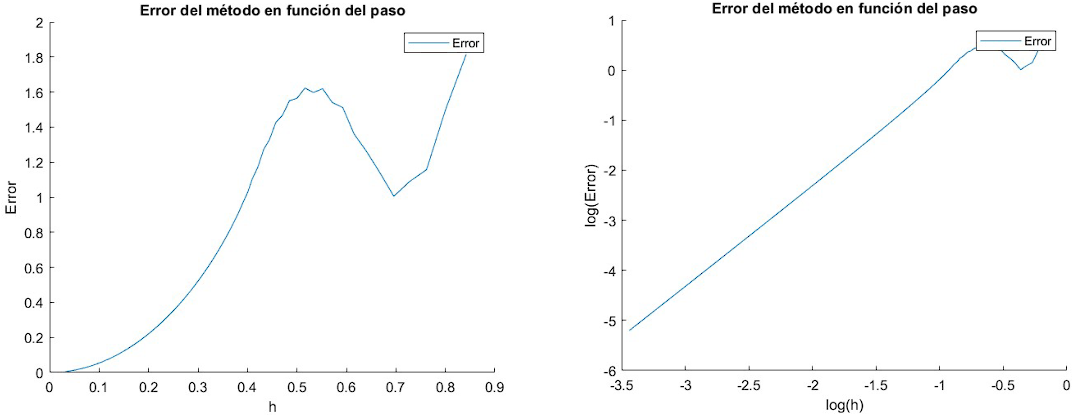
\includegraphics{fotos/errorosciladorenegias.png}
    \end{adjustbox}
    \caption{A la izquierda la raíz del error cuadrático medio en las energías (Error), según el paso (h). A la derecha, el logaritmo de la raíz del error cuadrático medio en las energías (~log(Error)~), según el logaritmo del paso (~log(h)~).}
\end{figure}

     \subsubsection{Error en las funciones}

    Ahora mostraremos la evolución del error en las funciones en función, como anteriormente, del paso. Aclaramos aquí que se elige el método de Simpson para normalizar las autofunciones que comparamos con las analíticas. Los valores de N permanecen igual que para el apartado de las energías (de 10 a 500).

\begin{figure}[H]
    \centering
    \begin{adjustbox}{width=1.2\linewidth,center}
        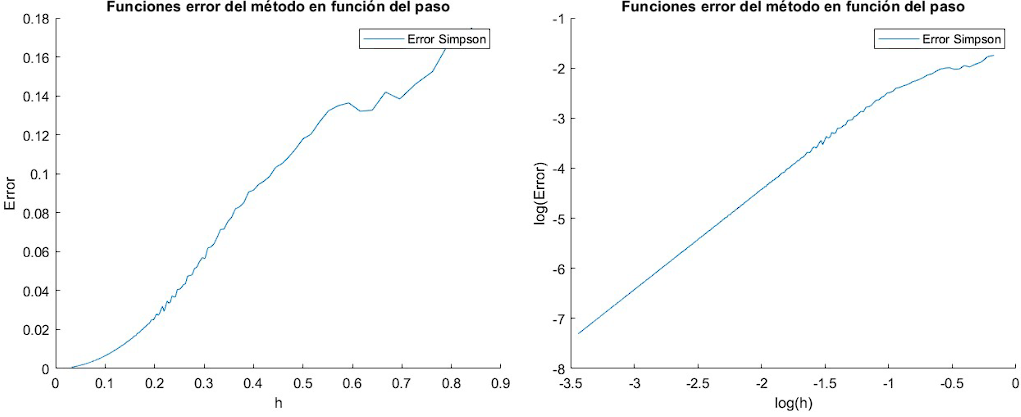
\includegraphics{fotos/errorfuncionseoscilador.png}
    \end{adjustbox}
    \caption{A la izquierda la raíz del error cuadrático medio en las funciones (Error), según el paso (h). A la derecha, el logaritmo de la raíz del error cuadrático medio en las funciones (~log(Error)~), según el logaritmo del paso (~log(h)~).}
\end{figure}
        
\subsection{Pozo de potencial finito}

\subsubsection{Error en las energías}

Como ya se ha comentado con anterioridad, las energías 
que se presentan como analíticas son una aproximación ya que 
no hay ninguna forma de obtener su valor numérico. Por esta
razón, el error que obteníamos era bastante alto en comparación
con los otros dos potenciales. \\

Es por esto que hemos optado por no hacer el estudio de errores para estas energías debido a que al no tener una solución real completamente precisa el error va bajando, como es lógico, pero nunca va a llegar a 0. Es por esto que hemos considerado que no tiene sentido comparar un método numérico con una aproximación ya que, evidentemente, el error jamás convergerá a 0.

\subsubsection{Error en las funciones}

Para este apartado sí disponemos de soluciones exactas y es 
por ello que vamos a realizar el correspondiente estudio de la 
evolución de su error. \\

Para realizar este estudio, al igual que en el resto de secciones, 
se ha decidido usar el método de Simpson para normalizar las 
autofunciones y un N que abarca los valores de 10 a 500. 
También, al igual que sucedía en el pozo de potencial 
infinito, nuestras soluciones presentas oscilaciones y hemos 
vuelto a usar un gráfico de dispersión al que le hemos realizado 
un ajuste.

\begin{figure}[H]
    \centering
    \begin{adjustbox}{width=1.2\linewidth,center}
        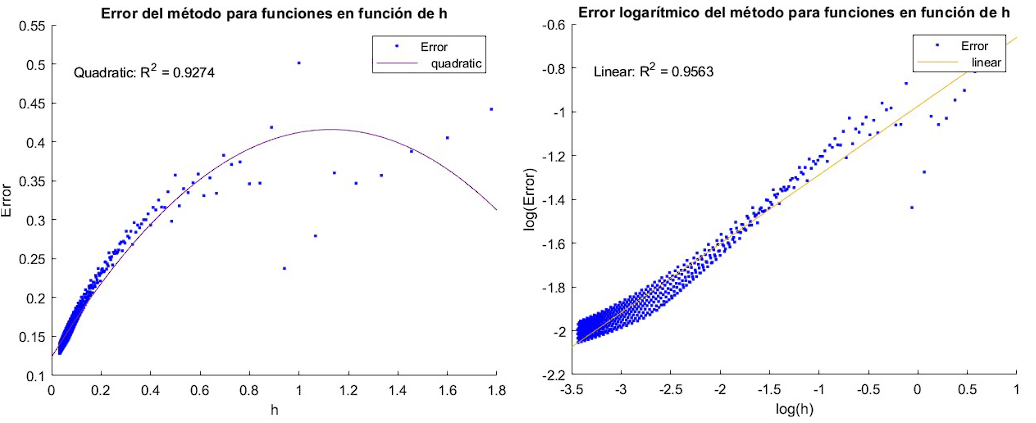
\includegraphics{fotos/errorfinitofunciones.png}
    \end{adjustbox}
    \caption{A la izquierda la raíz del error cuadrático medio en las funciones (Error), según el paso (h). A la derecha, el logaritmo de la raíz del error cuadrático medio en las funciones (~log(Error)~), según el logaritmo del paso (~log(h)~).}
\end{figure}

\newpage
Como se puede apreciar, en la primera gráfica podemos concluir
que, a pesar de que el ajuste que se haya usado ha sido uno 
cuadrático, el error se comporta como cabría esperar (logarítmico).
Sin embargo, por algunos datos atípicos, esa forma que cabría esperar encontrarse se deforma un poco. \\

Por otra parte, si nos fijamos en el error en logaritmos, 
vemos que una linea recta lo aproxima muy bien. Con lo cual, 
podemos considerar como acertado los métodos de integración usados
para normalizar. \\

Por último, observar que si siguiéramos aumentando el número de puntos usados, el error acabaría llegando a 0, por lo que podemos estar satisfechos con los resultados obtenidos.

\subsection{Métodos de integración}

    Esta sección es de verdadero interés pues representa un tipo de inconveniente que nos hemos encontrado realizando el trabajo. Nuestro código es capaz de realizar la normalización de las autofunciones tanto con el método de los trapecios como con el de Simpson. Sin embargo, cuando representamos la convergencia de uno frente a la de otro nos encontramos con lo siguiente:

\begin{figure}[H]
    \centering
    \begin{adjustbox}{width=1.2\linewidth,center}
        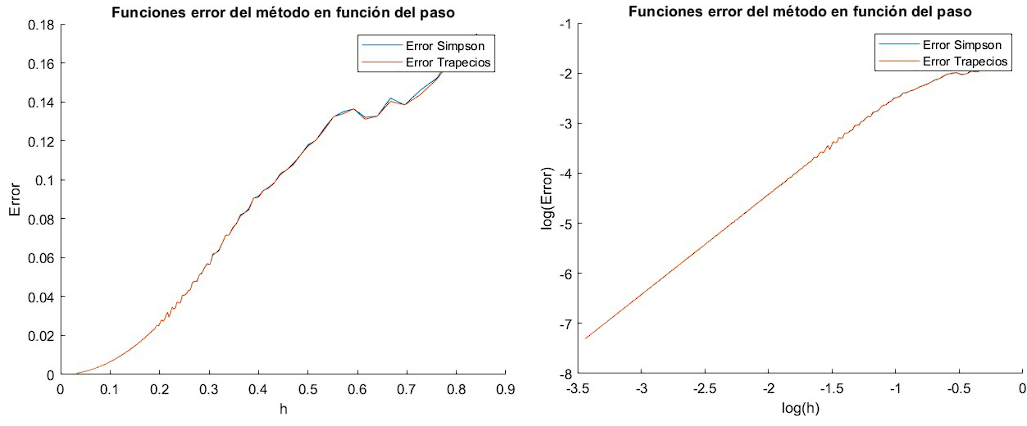
\includegraphics{fotos/comparacionsimpsontrapecios.png}
    \end{adjustbox}
    \caption{A la izquierda el error de ambos métodos en función del paso. A la derecha la misma gráfica pero tomando logaritmos en las variables de los ejes.}
\end{figure}

¡Nos encontramos con que ambos métodos nos ofrecen la misma convergencia! ¿Como es esto posible?, el error del método de Simpson es de orden $h^4$ mientras que el de trapecios va como $h^2$. Después de comprobar si existían errores que pudieran llevar a conclusiones equivocadas, encontramos un motivo del por qué esto puede ser así.\\

Cuando el método de diferencias finitas nos devuelve las autofunciones sin normalizar, estas ya poseen un error asociado  este método numérico, precisamente de orden $h^2$. Nosotros realizamos la normalización de estos autovectores con dos métodos distintos, sí, pero en ambos casos esos vectores salen del mismo sitio, y por tanto, con el mismo error de procedencia.\\

Esto puede provocar entonces que los dos métodos de integración se comporten igual a la hora de normalizar y desde luego explicaría la razón de por qué al graficar el error de uno frente al del otro ambos se comporten de manera similar.
    
\section{Consideraciones: Ecuación dependiente del tiempo}

Es importante mencionar que una vez resuelta nuestra ecuación independiente del tiempo ahora nos sería posible resolver la ecuación dependiente del tiempo. Esta ecuación es:

\begin{equation*}
    i\hbar \frac{\partial}{\partial t} \Psi(x, t) = -\frac{\hbar^2}{2m} \frac{\partial^2}{\partial x^2} \Psi(x, t) + V(x, t) \Psi(x, t)
\end{equation*}

\begin{equation*}
    i\hbar \frac{\partial}{\partial t} \Psi(x, t) = H \Psi(x, t)
\end{equation*}

\begin{equation}
    i\hbar \frac{\partial}{\partial t} \Psi(x, t) = E \Psi(x, t)
\end{equation}

Vemos que en esta ecuación ya conocemos las energías debido a que estas son invariantes en el tiempo, por tanto, nuestro problema se convierte en el cálculo de una ecuación diferencial.
Para resolverlo podemos usar por ejemplo el método de Runge-Kutta, estableciendo como condiciones iniciales las funciones de onda a tiempo $t=0$ : $\Psi(x,0)$. Estas serán nuestras funciones $\Psi(x)$ ya que si suponemos las soluciones estacionarias:

\[
    \Psi(x,t)=\Psi(x)g(t)
    \]

entonces:

\[
    g(t)=e^{\frac{i}{\hbar}Et} \,\,\rightarrow\,\, g(0)=1
\]

y por tanto:

\[
    \Psi(x,0)=\Psi(x)
\]




\newpage
\section{Anexo}
\subsection{Códigos de MATLAB y enlace a GitHub}
Adjunto con este trabajo, se envía el fichero de archivos que se ha utilizado para realizar todas las simulaciones descritas aquí, tanto las pertinentes a graficar las soluciones como las que se encargan de realizar el análisis de errores.\\

Con el objetivo de que el código sea reutilizable y capaz de estudiar las soluciones de la Ecuación de Schrödinger independiente del tiempo, se ha realizado a modo de interfaz un script en concreto que ha de ejecutarse en pos de observar lo que el usuario desee.\\

Este script inicial es \textit{THE\_MAIN.m}, el cual a la hora de ejecutarse le pedirá al usuario lo que desea visualizar, haciéndole elegir entre realizar un estudio de:

\begin{itemize}
    \item Soluciones: El usuario entonces deberá ingresar los límites del dominio, el número de puntos con los que dividir el espacio y el número de autofunciones que debe mostrar.

    \item Errores: A lo anterior hay que añadirle el número mínimo de puntos (el cual no debe ser inferior a 10) y el máximo para ver como evoluciona el error según el paso de discretización (a menos puntos, mayor el paso). Como se enseñará el error en las energías y el error en las funciones, para este segundo el programa también pedirá si la normalización se hará mediante el método de los trapecios o mediante el método de Simpson.

\end{itemize}

Además, como recurso adicional, todo el contenido del trabajo se puede encontrar en un repositorio de GitHub que hemos creado para este trabajo. El acceso al mismo se puede realizar a través del siguiente enlace:

\begin{center}
    \href{https://github.com/JavierZeta/Schrodinguer-equation-}{Repositorio Schrödinger Equation}
\end{center}

\nocite{*}
\printbibliography

\end{document}
